
\documentclass[a4paper, 12pt]{article}
%\usepackage{mathtext}
\usepackage{cmap}
\usepackage[english, russian]{babel}
\usepackage[T2A]{fontenc}
\usepackage[utf8]{inputenc}
\usepackage[left=2cm, right=1.5cm, top=2cm, bottom=2cm]{geometry}
\usepackage{amsmath}
\usepackage{amssymb}
\usepackage{etoolbox}
\usepackage{amsthm}
\usepackage{amsfonts}
\usepackage{mathtools}
%\usepackage{indentfirst}
\usepackage{soulutf8}
\usepackage{graphicx}
%


\usepackage{tikz,amstext}
\newlength{\tempheight}
\newcommand{\Let}[0]{%
\mathbin{\text{\settoheight{\tempheight}{\mathstrut}\raisebox{0.5\pgflinewidth}{%
\tikz[baseline,line cap=round,line join=round] \draw (0,0) --++ (0.4em,0) --++ (0,1.5ex) --++ (-0.4em,0);%
}}}}

\newcommand{\R}{\mathbb R}
\newcommand{\Q}{\mathbb Q}
\newcommand{\Z}{\mathbb Z}
\newcommand{\N}{\mathbb N}
%\newcommand{\C}{\mathbb C}
\renewcommand{\phi}{\varphi}
\renewcommand{\epsilon}{\varepsilon}
\newcommand{\aug}{\fboxsep=-\fboxrule\!\!\!\fbox{\strut}\!\!\!}
\newcommand\tab[1][.5cm]{\hspace*{#1}}
\newcommand\undermat[2]{\makebox[0pt][l]{$\smash{\underbrace
{\phantom{\begin{matrix}#2\end{matrix}}}_{\text{$#1$}}}$}#2}
\newcommand\overmat[2]{\makebox[0pt][l]{$\smash{\overbrace
{\phantom{\begin{matrix}#2\end{matrix}}}^{\text{$#1$}}}$}#2}

\newcounter{lemcount}
\newcounter{thcount}
\theoremstyle{definition}
\newtheorem*{definition}{Определение}
\newtheorem*{theorem}{Теорема}
\newtheorem*{consequense}{Следствие}
\newtheorem*{lemma}{Лемма}
\newtheorem*{subtheorem}{Утверждение}
\newtheorem*{remark}{Замечание}
\newtheorem*{example}{Примеры}
\newtheorem*{example1}{Пример}
\newtheorem*{lalala}{Упражнение}
\newtheorem*{algorithm}{Алгоритм}
\newtheorem*{properties}{Свойства}
\newtheorem*{properties1}{Свойство}
\newtheorem{lemmanum}[lemcount]{Лемма}
\newtheorem{theoremnum}[thcount]{Теорема}
\newtheorem{theoremL}{Теорема}[section]

\usepackage[russian]{babel}
\addto\captionsenglish{% Replace "english" with the language you use
  \renewcommand{\contentsname}%
    {Содержание}%
}

\usepackage{titlesec}
\titleformat{\section}{\LARGE \bfseries}{\thesection}{1em}{}
\titleformat{\subsection}{\Large\bfseries}{\thesubsection}{1em}{}
\titleformat{\subsubsection}{\large\bfseries}{\thesubsubsection}{1em}{}

\usepackage{hyperref}
\usepackage{xcolor}
% Цвета для гиперссылок
\definecolor{linkcolor}{HTML}{225ae2} % цвет ссылок
\definecolor{urlcolor}{HTML}{225ae2} % цвет гиперссылок
\hypersetup{
    pdfstartview=FitH, 
    linkcolor=linkcolor,
    urlcolor=urlcolor,
    colorlinks=true
}

\begin{document}
  \begin{titlepage}
    \newpage
    
    \begin{center}
    
\includegraphics[width=4cm]{image/image.png}
    \end{center}
    
    \vspace{4em}
    
    \begin{center}
    \Large Механико-математический факультет  
    \end{center}
    
    \vspace{2em}
    
    \begin{center}
    \large{\textsc{\textbf{Алгебра, 1 семестр, 2 поток}}}
    \end{center}
    
    \vspace{6em}
    

    
    \newbox{\lbox}
    \savebox{\lbox}{\hbox{Молчанов Вячеслав Вадимович}}
    \newlength{\maxl}
    \setlength{\maxl}{\wd\lbox}
    \hfill\parbox{11cm}
    {
    \hspace*{5cm}\hspace*{-5cm}Преподаватель:\hfill\hbox to\maxl{Куликова Ольга Викторовна\\} \\

    \hspace*{5cm}\hspace*{-5cm}Студент:\hfill\hbox to\maxl{Молчанов Вячеслав\\}\\

    \hspace*{5cm}\hspace*{-5cm}Группа:\hfill\hbox to\maxl{108} \\
    
    \hspace*{5cm}\hspace*{-5cm}Контакт:\hfill\hbox to\maxl {\href{https://t.me/Slavikvaxye}{Мой телеграм для связи \\}}
    }

    \vspace{\fill}
    
    \begin{center}
    Москва \\2024 
    \end{center}
  \end{titlepage}
  \tableofcontents
  \fontsize{14pt}{20pt}\selectfont
  \newpage
  \fontsize{14pt}{20pt}\selectfont
  \section{Система линейных уравнений}
  \subsection{Матрица. Основные понятия}
  \begin{definition}
    Матрица $A$ размера $m\times n$ это прямоугольная таблица с $m$ строками и $n$ столбцами
    $$ A= \begin{pmatrix}
      a_{11} && a_{12} && \dots && a_{1n}\\
      a_{21} && a_{22} && \dots && a_{2n}\\
      \vdots && \null && \null && \vdots\\
      a_{m1} && a_{m2} && \dots && a_{mn}
    \end{pmatrix}$$ \\
    $a_{ij}$ - элемент матрицы и индексы:

    \begin{itemize}
      \item $i$ - номер строками
      \item $j$ - номер столбца
    \end{itemize}
    
    $M_{m\times n}(\R)$ - Множество всех матриц размера $m\times n$ с элементами из $\R$
    \end{definition}
    Матрица $m\times 1$ называется столбцом:
    $$ A= 
    \begin{pmatrix}
      a_{11} \\
      a_{21} \\
      \vdots \\
      a_{m1} 
    \end{pmatrix} $$
    Если $A=(a_{ij})$ - крадратная, $a_{ij} = 0\ \forall i \neq j$, то $A$ называется диальнольной.
    $$ A =
    \begin{pmatrix}
      a_{11} && \null && \null && 0 \\
      \null && a_{22} && \null && \null \\
      \null && \null && \ddots && \null \\
      0 && \null && \null && a_{nn} 
    \end{pmatrix} $$

    Если $A$ - диальнольная и $a_{ij}$ = 1, то $A$ называется единичной.
    $$ A =
    \begin{pmatrix}
      1 && \null && \null && 0 \\
      \null && 1 && \null && \null \\
      \null && \null && \ddots && \null \\
      0 && \null && \null && 1 
    \end{pmatrix} $$

    \newpage
    %%%%%%%%
    Если $A$ - квадратная, то
    \begin{itemize}
      \item $ A =\begin{pmatrix}
        a_{11} && \null && \null \\
        \null && \ddots && \null \\
        \null && \null && a_{nn} 
      \end{pmatrix} $ главная диагональ
      \item $ A =
      \begin{pmatrix}
        \null && \null && a_{n1} \\
        \null && \dots && \null \\
        a_{n1}  && \null && \null
      \end{pmatrix} $ побочная диагональ
    \end{itemize}
    
    \begin{definition}
      Если $A$ - размера $m\times n$, $a_{ij} = 0\ \forall i,j$, то $A$ называется нулевой.
    \end{definition}

    \subsection{Система линейных (алгебраческих) уравнений}
    $(*)
    \begin{cases}
      a_{11}x_1 + ... + a_{1n}x_n = b_1 \\ 
      a_{21}x_2 + ... + a_{2n}x_n = b_2 \\
      \vdots \\
      a_{n1}x_1 + ... + a_{nn}x_n = b_n
    \end{cases}$ $\\$$\\$
    где $a_{ij}, b \in \R, x_1,... ,x_n$ - неизвестные.
    $$A = \begin{pmatrix}
      a_{11} && \dots && a_{1n} \\
      \vdots && \null && \vdots \\
      a_{n1} && \dots && a_{nn} 
    \end{pmatrix} \hspace{30pt} B = \begin{pmatrix}
      a_{11} \\
      \vdots \\
      b_{n}
    \end{pmatrix}$$
    $A$ - матрица коэфициентов, $a_{ij}$ называется коэфициентом СЛУ.\\
    $B$ - столбец свобоных членов, $b_{j}$ - свободный член.
    \begin{definition}
      Расширенная матрица $\underset{m\times (n+1)}{(A|B)}$. Набор чисел $x_1^0,...,x_n^0 \in \R$ называется решением системы $(*)$, если подстановка этих чисел вместо неизвестных в $(*)$ дает тождество в каждом уравнении. $(x_i^0\longleftrightarrow x)$ 
    \end{definition}
    Решить систему - это найти все решения системы. Любое конткретное решение называется частным.
    \begin{definition}
      Если СЛУ имеет решение, то она называется совместной, иначе несовместной. 
    \end{definition}  
    \begin{definition}
      Совместная система, имеющая одно решение, называется определенной, иначе неопределенной (более одного решения).
    \end{definition}  

    \newpage
    %%%%%%%%
    \subsection{Элементарные преобразования над СЛУ}
    \begin{enumerate}
      \item Прибавить к одному уравнению другое уравнение, умноженное на число $\lambda \in \R$
      \item Поменять местами два уравнения
      \item Умножить уравнение на ненулевое число $\mu \in \R$
    \end{enumerate}
    \begin{subtheorem}
      Эти преобразования обратимы.
    \end{subtheorem}
    \begin{definition}
      Две системы линеных уравнений называются эквивалентными, если их множества решений совпадают.
    \end{definition}
    \begin{subtheorem}
      Если одна СЛУ получена из другой СЛУ с помощью конечного числа элементарных преобразований, то эти системы эквивалентны.
    \end{subtheorem}
    \begin{proof}
      $ \\ \Longrightarrow$ (Не Куликова) 
      $AX = B$ - исходная система, $\tilde{A} X = \tilde{B}$ преобразованная система. \\
      Пусть ${z_1,...,z_n}$ некотороое решение $AX = B$. Будем рассматривать $\tilde{A} X = \tilde{B}$, в ней ЭП $II$ типа умножают строку на $\mu$, имеем:
      $$a_{i1}x_1 +...+ a_{in}x_n = b_{i} \text{ в } AX = B$$
      $$\mu a_{i1}x_1 +...+\mu a_{in}x_n = \mu b_i \text{ в } \tilde{A} X = \tilde{B}$$ 
      Выносим $\mu$ из второго уравнения:
      $$\mu (a_{i1}x_1 +...+ a_{in}x_n) = \mu b_i$$
      Получаем, что ${z_1,...,z_n}$ решение для $\tilde{A} X = \tilde{B}$. Для $III$ типа ЭП очевидно. Теперь рассмотрим $I$ тип, будем к i-ой строчке прибавлять j-ую к коэфициентом $\lambda$, получаем:
      \begin{multline*}
      (a_{i1}+\lambda a_{j1})x_1 +...+(a_{in}+\lambda a_{jn})x_n = \\ = a_{i1}x_1+\lambda a_{j1}x_1 +...+a_{in}x_n+\lambda a_{jn}x_n = \tab[3cm] \\ = a_{i1}x_1 + ... + a_{in}x_n + \lambda (a_{j1}x_1 +...+ a_{jn}x_n) = b_i + \lambda b_j
      \end{multline*}
      Таким образом, любое решение старой СЛУ - это и решение новой, то есть множество
      решений не уменьшилось. (со столбцами все тоже самое) \\
      $\Longleftarrow$ В обратную сторону аналогично (для доказательства эквивалентности), используя обратимость элементарных преобразований.
    \end{proof}
    Мораль в том, что мы можем работать с расширенной матрицей $(A|B)$.

    \newpage
    %%%%%%%%
    \subsection{Элементарные преобразования над матрицами}
    \textbf{Элементарные преобразования над строками:} 
    $$A =\begin{pmatrix}
      \overline{a_1} \\
      \overline{a_2} \\
      \vdots \\
      \overline{a_i}
    \end{pmatrix}, \text{ где } \overline{a_i} - \text{строка}$$
    \begin{itemize}
      \item ЭП1: $\overline{a_i} \to \overline{a_i} + \lambda \overline{a_i}$
      \item ЭП2: $\overline{a_i} \longleftrightarrow   \overline{a_j}$
      \item ЭП3: $\overline{a_i} \to \mu \overline{a_i},\ \mu \neq 0$
  \end{itemize}
  \begin{definition}
    Лидер строки (ведущий элемент) - это 1-й ненулевой элемент слева. \\
    \textbf{Пример:} $(0, 0, \underbrace{3}_{\text{лидер}}, 4, 5, 0, 0, 7)$
  \end{definition}
  \begin{definition}
    Матрица $A$ размера $m\times n$ называется ступенчатой, если 
    \begin{enumerate}
      \item Номера лидеров ненулевых строк строго возрастают с увеличением номера строки.
      \item Все нулевые строки стоят внизу (в конце).
    \end{enumerate}
  \end{definition}
  \begin{theorem}
    Любую матрица $A$ размера $m\times n$ за конечное число элементарных преобразований над строками можно привести к ступенчатому виду.
  \end{theorem}
  \begin{proof} Индукция по $n$: \\
    Если $A$ - нулевая, то $A$ - ступенчатого вида. Если $A \neq 0$ : найдем первый ненулевой столбец (начиная слева). Пусть $j$ - номер первого ненулевого столбца. Пусть $a_{ij} \neq 0$: 
    $$A =\begin{pmatrix}
      0 && 0 && \null && \null  \\
      \vdots && \vdots && \null  \\й
      \null && \null && a_{ij} && \null \\
      \vdots && \vdots && \null  \\
      0 && 0 && \null && \null  \\
    \end{pmatrix}$$ 

    \newpage
    %%%%%%%%
    Меняем 1-ю и $i$-ю строку местами и получаем, что $a_{ij}$ стал лидером первой строки. Считаем, что сразу $a_{1j} \neq 0$:
    $$A = \begin{pmatrix}
      0 && 0 && a_{ij} && * \\
      \vdots && \vdots && * && *  \\
      \null && \null && \vdots && \null \\
      \vdots && \vdots && \vdots && \null  \\
      0 && 0 && \vdots && \null  \\  
    \end{pmatrix} $$ \\
    Вычитаем из кажкой $k$-й строки, начиная со 2-ой, 1-ю строку, умноженную на число $\frac{a_{kj}}{a_{1j}}$. Получает вид: 
    $$\tilde{A} =\begin{pmatrix}
      0 && 0 && \vline && * && \null \\
      \vdots && \vdots && \vline && * && * \\
      \null && \null && \vline && \vdots && \null \\
      \vdots && \vdots && \vline && \vdots && \null  \\
      0 && 0 && \vline && \vdots && \null  \\
    \end{pmatrix}$$ \\
    К правой части матрицы применяем индукцию и проводим матрицу к ступенчатому виду.
  \end{proof}
  \begin{remark}
    Этот метод называется  методом Гауса.
  \end{remark}

  \subsection{Решение СЛУ методом Гауса}
  $\begin{cases}
    a_{11}x_1 + ... + a_{1n}x_n = b_1 \\ 
    a_{21}x_2 + ... + a_{2n}x_n = b_2 \\
    \vdots \\
    a_{m1}x_1 + ... + a_{mn}x_n = b_m
  \end{cases}$ \\$\\$
  Элементарные преобразования над $AX=B$ $\Longleftrightarrow$ элементарные преобразования над $(A|B)$. 

  СЛУ $AX=B$ ступенчатая $\Longrightarrow $ $(A|B)$ имеет ступенчатый вид.

  \newpage
  %%%%%%%%
  \begin{subtheorem}
    Решение СЛУ ступенчаного вида.
  \end{subtheorem}  
  Пусть $AX=B$ - ступенчатая
  $$(A|B)=\begin{pmatrix}
    a_{11} & \null & \null & \null & \vline & b_1 \\
    \null & a_{22} & \null & \null & \vline & \vdots \\
    \null & \null & \ddots & \null & \vline & \vdots \\
    \null & \null & \null & a_{sn} & \vline & b_s \\
    \null & \null & \null & \vdots & \vline & \vdots \\
    0 & \cdots & \cdots & 0 & \vline & b_{\widetilde{s}}
  \end{pmatrix}$$ \\
  $\widetilde{s}$ - ненулевые строки расширенной матрицы \\
  s - число ненулевых строк 

  $\widetilde{s}=\left[
    \begin{gathered}
      s \\
      s+1
    \end{gathered}
  \right.$


  \begin{itemize}
    \item[1 случай:]
    $\widetilde{s} \neq s \ (\widetilde{s}=s+1)$ \\ 
    Рассмотрим последнюю ненулевую строку:
    $$\begin{pmatrix}
      a_{11} & \null & \null & \null & \vline & b_1 \\
      \null & a_{22} & \null & \null & \vline & \vdots \\
      \null & \null & \ddots & \null & \vline & \vdots \\
      \null & \null & \null & a_{sn} & \vline & b_s \\
      0 & \cdots & \cdots & 0 & \vline & b_{s+1}
    \end{pmatrix}$$ \\
    $0x_1+...+0x_n=b_{s+1}$ 
    $\Longrightarrow$ решение у этого уравнения нет 
    $\Longrightarrow$ СЛУ не имеет решения, т.е. несовместнаю. \\
    Далее $\widetilde{s}=s$\\
    Заметим, что $\widetilde{s}=s\leq n$ (n-количество столбцов)
    \item[2 случай:] $\widetilde{s}=s=n$  
    $$\left\{ \begin{aligned}
      a_{11} x_1 + a_{12} x_2+ \dots + a_{1n} x_n = b_1 \\
      a_{22} x_2 + \dots + a_{1n} x_n = b_2 \\ 
      \ddots \ \ \ \ \ \ \ \ \ \ \ \ \ \ \ \ \vdots \ \\
      a_{nn} x_n = b_n
    \end{aligned}
    \right.$$

    Такая СЛУ называются строго треугольной

    Из n-го уравнения однозначно находится $x_n = \frac{b_n}{a_{nn}}$
    Подставляем во все оставшиеся уравнения $x_n = \frac{b_n}{a_{nn}}$ $\Longrightarrow$ исключаем $x_n$. Получаем строго треугольную систему с меньшим количество неизвестных.  \\
    Далее из (n-1)-го уравнения  находим $x_{n-1}$ и т.д. $\Longrightarrow$ СЛУ имеет единственное решение т.е. является определенной.

    \item[3 случай:] $\widetilde{s}<n$ 
  $$\begin{pmatrix}
    0 & \null & 0 & |\underline{a_{1k_1}} & \ast & \cdots & \cdots & \ast & \vline & \ast  \\
    0 & \null & 0 & 0 & |\underline{a_{2k_2}} & \ast & \cdots & \ast & \vline & \ast \\
    \null & \null & \null & \null & \null & \ddots & \null & \null & \vline & \vdots
  \end{pmatrix}$$ 

  $a_{1k_{1}},...,a_{sk_{s}}$  - лидеры; \\
  $x_{k_{1}},...,x_{k_{s}}$ - главные неизвестные (неизвестные соответствуют лидерам) \\
  Оставшиеся неизвестные назовем свободными. \\
  Перекинем в правую часть СЛУ слагаемые, соответствующие свободным неизвестным 
  $\Longrightarrow$ получаем относительно главных неизвестных строго треугольную СЛУ. \\
  Как в случае 2 однозначно выражается главные неизвестные через свободные
  $\Longrightarrow$ с точностью до нумерации получаем:
  $$\begin{cases}
    x_1 = c_{1,s+1}x_{s+1} + \dots + c_{1n}x_n+d_1 \\
    \vdots \\
    x_s = c_{s,s+1}x_{s+1} + \dots + c_{sn}x_n+d_s
  \end{cases}$$   
  
  Это выражение называется общим решением системы. Подставляя вместо свободных неизвестных конкретное число из $\R$, получаем значение для главных. \\
  $\Longrightarrow$ получаем все решения СЛУ\\
  Если СЛУ имеет > 1 решения - такая СЛУ называется неопределенной. 
  \end{itemize}
  $$\begin{matrix}
    \null &&& \null && \ \ \text{\ \ \ \ СЛУ} \\
    \null && \null && \swarrow && \searrow \\
    &&& \widetilde{s} \neq s && \null &&\widetilde{s} = s\\
    \null &&& \text{несовместна} && \null && \text{совместна} \\
    \null && \null && \null && \swarrow \null && \searrow \\
    \null && \null && \null && \widetilde{s} = s = n \null && \widetilde{s} = s \leq n \\
    \null && \null && \null && \text{определенна} \null && \text{неопределенна}
  \end{matrix}$$
  \begin{algorithm}
    $AX=B \longmapsto (A|B) \thicksim (A_{c}|B_{c})\longmapsto A_cX=B_c$
  \end{algorithm}

  \newpage
  %%%%%%%%
  \begin{definition} 
    Матрица $A$ имеет улучшенный ступенчатый вид, если выполнены следующие условия:
    \begin{enumerate}
      \item $A$ - ступенчатого вида
      \item Все лидеры равны 1
      \item В каждом столбце, где есть лидер $\neq 0$ , все элементы равны 0 
    \end{enumerate}
  \end{definition}  

  \begin{subtheorem}
    Любую матрицу $A$  можно привести к улучшенному ступенчатому виду с помощью элементарных преобразований.
  \end{subtheorem} 
  \begin{proof}
    Т.к. любую матрицу можно привести к ступенчатому виду $\Longrightarrow$ будем считать, что $A$ - ступенчатая. \\
    Рассмотрим последний лидер $a_{sk_s}$. Если $a_{sk_s} \neq 1$, то s-ю строку делим на $a_{sk_s}$ и получаем, что $\widetilde{a_{sk_s}}=1$. \\ Далее из всех строк вычитаем первую, умноженную на $a_{ik_s} \Longrightarrow \widetilde{a_{ik_s}}  =0$ и т.д. 
  \end{proof} 

  \begin{definition}
    СЛУ $AX=B$ называется однородной, если $B=0$, т.е. все свободные члены нулевые.  
  \end{definition} 
  \begin{subtheorem}
    Однородная система всегда совместна.
  \end{subtheorem} 
  \begin{proof}
    $AX=0$ всегда имеет решение $x_1=0,...,x_n=0$ (тривиальное решение)
  \end{proof} 
  \begin{consequense}
    Однородная СЛУ, в которой число уравнений $<$ числа неизвестных, имеет нетривиальное решение.  
  \end{consequense} 
  \begin{proof}
    (в обозначениях из метода Гаусса)\\
    Т.к. система совместна (т.к. $B=0$), то $s=\widetilde{s}$ \\
    С другой стороны $s=\overline{s} \leq$ число исходных уравнений $<$ n $\Longrightarrow s=\widetilde{s} < n \Longrightarrow$ СЛУ неопределенна $\Longrightarrow \exists$ более одного решения $\Longrightarrow \exists$ нетривиальное решение.     
  \end{proof} 

  \newpage
  %%%%%%%%
  \section{Векторные пространства}
  \subsection{Аксиомы элементов векторного пространства}
  Мы рассматриваем векторные пространства над полем $\R$.
  \begin{definition}
    Векторным пространством над $\R$ называют множество элементов $V$, на котором введены операции сложения и умножения на числа из $\R$:
    \begin{enumerate}
      \item $ \forall x,y \in V \Longrightarrow x+y=z \in V$
      \item $\forall \lambda \in \R, \forall x \in V \Longrightarrow \lambda x = w \in V$ 
    \end{enumerate}
    Удовлетворяет следующими свойствами:
    \begin{enumerate}
      \item $x+y = y+x$ (коммутативность)
      \item $(x+y)+z = x+(y+z)$ (ассоциативность)
      \item $\exists \tab[0.1cm] 0 \in V: \forall x \in V: x+0 = 0+x = x$ (нейтральный элемент относильно сложения)
      \item $\forall x \in V: \exists \tab[0.1cm] x^{\prime}: x + x^{\prime} = 0$ (противоположный элемент)
      \item $\forall \lambda \in \R, \forall x,y \in V: \lambda (x+y) = \lambda x + \lambda y$ (дистрибутивность умножения отностильно сложения)
      \item $\forall \lambda, \mu \in \R, \forall x \in V: (\lambda+\mu)x = \lambda x + \mu x $ (дистрибутивность сложения отностильно умножения)
      \item $\forall \lambda, \mu \in \R, \forall x \in V: \lambda(\mu x) = (\lambda \mu) x $ (ассоциативность умножения)
      \item $\forall x \in V: 1 \cdot x = x$ (нейтральный элемент относильно умножения)
    \end{enumerate}
  \end{definition} 

  \begin{definition}
    Любой элемент векторного пространства называется вектором.
  \end{definition} 

  \textbf{Примеры векторных пространств:} 
    \begin{enumerate} 
      \item $V^2$ - Геометрические векторы на плоскости.
      \item $V^3$ - Геометрические векторы в пространстве.
      \item $\R^n$ = $\{ {(a_1,...,a_n) | a_i \in \R} \}$ - арифметические векторы.
    \end{enumerate}
    \tab[0.8cm]"$+$": $(a_1,...,a_n)$ + $(b_1,...,b_n)$ = $(a_1+b_1,...,a_n+b_n)$ \\
    \tab[0.8cm]"$\times$": $(a_1,...,a_n) \times \lambda$ = $(a_1\lambda,...,a_n\lambda)$ 
  \begin{lalala}
    Проверьте, что $\R^n$ (арифметическое пространство строк) с этими операциями является векторным пространством. 
  \end{lalala}  
  \subsection{Следствия}
  \begin{enumerate}
    \item нулевой вектор единственный
    \begin{proof}
      Пусть существует два $\overline{0}_1,\overline{0}_2 \in V$, тогда: $$\overline{0}_2 = \overline{0}_1 + \overline{0}_2 = \overline{0}_2 + \overline{0}_1 = \overline{0}_1$$   
    \end{proof} 
    \item $\forall x \in V$ противоположный вектор единственный
    \begin{proof}
      Пусть существует два $x_1,x_2$ - различные противоположные к вектору $x$, тогда:
      $$\overline{0} + x_2 = (x_1 + x) + x_2 = x_1 + (x + x_2) = x_1 + \overline{0}$$    
    \end{proof} 
    \item $\forall \lambda \in \R: \lambda \cdot \overline{0} = \overline{0}$ 
      \begin{proof}
      $$\lambda \cdot \overline{0} = \lambda \cdot (\overline{0}+\overline{0}) = \lambda \cdot \overline{0} + \lambda \cdot \overline{0}$$ Прибавим к обе им частям уравнения $\lambda \cdot \overline{0} = \lambda \cdot \overline{0} + \lambda \cdot \overline{0}$  противоположный к $\lambda \cdot \overline{0}$, тогда: $$\lambda \cdot \overline{0} + (-\lambda \cdot \overline{0})= \lambda \cdot \overline{0} + \lambda \cdot \overline{0} + (-\lambda \cdot \overline{0})$$ $$\overline{0} = \lambda \cdot \overline{0}$$ 
      \end{proof} 
    \item $\lambda \cdot (-x) = -\lambda \cdot x$
    \item $\lambda \cdot (x-y) = \lambda x - \lambda y$ 
    \item $(-1) \cdot x = -x$
    \item $(\lambda - \mu)\cdot x = \lambda x - \mu x$  
  \end{enumerate}
  \subsection{Векторные подпространства}
  \begin{definition}
    Подмножество $U\subseteq V$ называется векторным подпространством, если:
    \begin{enumerate}
      \item $ x, y \in U \Longrightarrow  x + y \in U$ 
      \item $\forall \lambda \in \R, \forall x \in U \Longrightarrow \lambda \cdot x \in U$ 
      \item $U \neq \varnothing$ 
    \end{enumerate}
  \end{definition} 
  \begin{remark}
    3 условие заменить на условие: $0 \in  U$
    \begin{itemize}
      \item [$\underline{\Longleftarrow}$] очевидно.
      \item [$\underline{\Longrightarrow}$] если $U \neq \varnothing$, то $\exists \tab[0.1cm] x \in U \Longrightarrow$ по $2.: (-1) \cdot x \in U \Longrightarrow -x \in U  \Longrightarrow \\ x + (-x) \in U \Longrightarrow 0 \in U$ 
    \end{itemize}
  \end{remark} 
  \begin{subtheorem}
    Любое векторное подпространство векторного пространства $V$ само является векторным пространством относительно операций векторного пространства $V$. 
  \end{subtheorem} 
  \begin{proof}
    Надо проверить определение. 1 и 2 свойство из операций \\ векторного пространства означают, что в $U$ заданы операции сложения и \\ умножения на вещественное число. Проверка аксиом векторного пространства: 1,2,5,6,7,8 - выполнены для всех векторов из $V$, а значит и для всех векторов из $U$. \\ 3,4 доказательство как в замечании: 
    $$\forall x \in U, \ \exists \tab[0.1cm](-x) = (-1) \cdot x \in U, \ \overline{0} \in U, \text{ т.к. } U \neq \varnothing $$   
  \end{proof} 
  \begin{example} \end{example}
    \begin{enumerate} 
      \item $V^3, U$ - множество всех векторов из $V^3$, параллельные фиксированной плоскости.
      \item $\R^n, U=\{(a_1,..., a_n) | a_{2i} = 0\}$ - векторное подпространство \\ $\widetilde{U} = \{(a_1,..., a_n) | a_{2i} = 1\}$ - не векторное подпространство, т.к. множество не замкнуто относительно сложения и умножения.
      \item В любом векторном простанстве $V$ есть такие подпространства, состоящие только из нулевого вектора. (тривиальное или несобственное подпространство) (Остальное называется собственными)
    \end{enumerate}
  
  \newpage
  %%%%%%%%
  \subsection{Линейная зависимость системы векторов}
  $V$ - векторное пространство над полем $\R$
  \begin{definition}
    Линейной комбинацией векторов $v_1,...,v_n \in V$ с коэфициентами $\lambda_1,...,\lambda_n \in \R$ называется выражение вида: 
    $$\lambda_1 x_1 + \cdots + \lambda_n x_n$$ 
    Говорят, что вектора $w \in V$ линейно выражаются через $(v_1,...,v_n)$, \\ если $\exists\tab[0.1cm]\lambda_1,...,\lambda_n \in \R: w = \lambda_1 x_1 + \cdots + \lambda_n x_n$   
  \end{definition}   
  \begin{definition}
    Линейная комбинация $\lambda_1 x_1 + \cdots + \lambda_n x_n$ называется тривиальной, если $\lambda_1 = 0,...,\lambda_n = 0$. Иначе нетривиальной.
  \end{definition}
  \begin{definition}
    Система векторов $v_1,...,v_n$ называется линейно зависимой (ЛЗ), если $\exists$ нетривиальная линейная комбинация равная 0, (т.е. $\exists \tab[0.1cm]\lambda_1,...,\lambda_n \in \R$ не все равные 0) такая что $\lambda_1 x_1 + \cdots + \lambda_n x_n = 0$. Иначе система называется линейно независимой (ЛНЗ), т.е. из любого такого равенства $\lambda_1 x_1 + \cdots + \lambda_n x_n = 0 \\ \Longrightarrow (\lambda_1,...,\lambda_n) = 0$.
  \end{definition}
  \begin{example}
    $V^2, v_1 = i + j, v_2 = 2i, v_3 = 3i$ -линейно зависимая система, т.к. $$1 \cdot (i + j) + (- \frac{1}{2}) \cdot (-\frac{1}{3}) \cdot (3i) = 0$$ $$1 \cdot v_1 + (-\frac{1}{2}) \cdot v_2 + (-\frac{1}{3}) \cdot v_3 = 0$$  
  \end{example}  
  \begin{properties} \end{properties} 
    \begin{enumerate}
      \item Система из одного вектора $V_1$ ЛЗ $\Longleftrightarrow V_1 = 0$  
      \item Система из 2-х векторов $v_1 \text{и } v_2$ ЛЗ $\Longleftrightarrow$ они пропорциональные, т.е. $v_1 = \lambda v_2 \\ v_2 = \mu v_1$. 
    \end{enumerate}
  \begin{example1}
    $\R^n$ \\
    Система $\underbrace{(1,0,0,...,0)}_{e_1} , \underbrace{(0,1,0,...,0)}_{e_2},...,\underbrace{(0,0,0,...,1)}_{e_n}$ линейно независимая \\
    $\lambda_1 e_1 + \cdots + \lambda_n e_n = (0,...,0) \Longleftrightarrow (\lambda_1,...,\lambda_n) = 0 \Longleftrightarrow $ ЛНЗ 
  \end{example1}
  \begin{lemmanum}
    (Критерий линейной зависимости)
    Система векторов $v_1,...,v_n \in V, \\ n>1$ - линейно зависимы $\Longleftrightarrow $ хотя бы один вектор линейно выражается через оставшиеся.  
  \end{lemmanum} 

  \newpage
  %%%%%%%%
  \begin{proof} $\tab$  
    \begin{itemize}
      \item[$\underline{\Longrightarrow}$]
      По определению ЛЗ $\exists \tab[0.1cm] \lambda_1,...,\lambda_n \in \R$ не все нулевые: $\lambda_1 v_1 + \cdots + \lambda_n v_n = 0$. Без ограничения общности можем считать, что $\lambda_1 \neq 0$, тогда $v_1 = \frac{1}{\lambda_1}(-\lambda_2 v_2 - \cdots - \lambda_n v_n)$
      \item[$\underline{\Longleftarrow }$] Пусть один из этих векторов выражается через оставшиеся. Без ограничения общности можем считать, что $v_1$ выражается через оставшиеся \\ $v_1 = \mu_2 v_2 + \cdots + \mu_n v_n$ \\ $1 \cdot v_1 -\mu v_2 - \cdots - \mu_n v_n = 0$ - нетривиальная линейнвая комбинация, \\ т.к. $\mu_1 (\text{коэф. перед }v_1) \neq 0 \Longrightarrow {v_1,...,v_n}$ - линейно зависима.
    \end{itemize}  
  \end{proof} 
  \begin{remark}
    В лемме 1 нельзя <<хотя бы один>> заменить на <<любой>>! \\
    Пусть $v_1 \neq 0, v_2 = 0$ и $v_1, v_2$ - ЛЗ, т.к. $0 \cdot v_1 + 1 \cdot v_2 = 0$
  \end{remark} 
  \begin{lemmanum} \label{lem2}
    Пусть $v_1,...,v_n \in V$ - ЛНЗ, тогда $w \in V$ линейно выражается через $v_1,...,v_n \Longleftrightarrow (w,v_1,...,v_n)$ - ЛЗ.   
  \end{lemmanum} 
  \begin{proof} $\tab$  
    \begin{itemize}
      \item[$\underline{\Longrightarrow}$] $\exists \tab[0.1cm] \mu_1,...,\mu_n \in \R: w = \mu_1 v_1 + \cdots +\mu_n v_n \Longrightarrow$ по критерию ЛЗ система $\{w,v_1,...,v_n\}$ - ЛЗ.
      \item[$\underline{\Longleftarrow}$] Пусть система ЛЗ $\Longrightarrow \exists \tab[0.1cm] \lambda_0,...,\lambda_n \in \R$ - не все нули, так что  $\lambda_0 w + \lambda_1 v_1 + \cdots + \lambda_n v_n = 0$, тогда: 
      \begin{enumerate}
        \item $ \lambda_0 = 0$, то $\lambda_1 v_1 + \cdots + \lambda_n v_n = 0$ - нетривиальная линейная комбинация
        \item $\lambda_0 \neq 0 \Longrightarrow w = (-\frac{\lambda_1}{\lambda_0})v_1 + \cdots + (-\frac{\lambda_n}{\lambda_0})v_n$
      \end{enumerate} 
    \end{itemize}
  \end{proof}
  %%
  \begin{lemmanum} \label{lem3}
    Пусть вектор $w$ линейно выражается через $v_1,...,v_k$. Тогда это выражение единственное.   
  \end{lemmanum} 
  \begin{proof} $\tab$ 
    \begin{enumerate}
      \item Пусть выражается единственно. Допустим, $v_1,..,v_k$ - ЛЗ $\Longrightarrow \exists\{\lambda_1,..,\lambda_k\}$ не все нулевые, т.ч. $\lambda_1v_1 + \cdots + \lambda_kv_k=0$ \\
      Тогда если $w=\mu_1v_1 + \cdots + \mu_kv_k$, то $w + 0 = (\mu_1+\lambda_1)v_1 + \cdots + (\mu_k + \lambda_k)v_k$ другое разложение, противоречие.  
      \item Пусть $v_1,..,v_k$ - ЛНЗ. Допустим, что существует два разложения: $$w = \mu_1v_1 + \cdots + \mu_kv_k$$  $$w = \widetilde{\lambda_1}v_1 + \cdots + \widetilde{\mu_k}v_k$$ 
      $\Longrightarrow  \{v_1,..,v_k\}$ - ЛЗ $\Longrightarrow $ противоречие.
    \end{enumerate}
  \end{proof}
  \begin{lemmanum} $\tab$
    \begin{enumerate}
      \item Если какая-то подсистема векторов ЛЗ, то вся система ЛЗ.
      \item Если система векторов ЛНЗ, то любая подсистема ЛНЗ.
    \end{enumerate}
  \end{lemmanum}  
  \begin{proof} $\tab$ 
    \begin{enumerate}
      \item Пусть подсистема $v_1,..,v_k$ системы $v_1,..,v_k,...,v_m$ - ЛЗ $\Longrightarrow \exists \lambda_1,...,\lambda_k$ не все равные нулю, т.ч. $\lambda_1v_1 + \cdots + \lambda_kv_k=0$ Положим $\lambda_{k+1}=0,...,\lambda_m=0$ 
      Тогда $\lambda_1v_1,..,\lambda_kv_k,...,\lambda_mv_m=0$ - нетривиальная ЛК $\Longrightarrow \{v_1,...,v_k,v_{k+1},...,v_m\}$ - ЛЗ. 
      \item Следует из 1.
    \end{enumerate}
  \end{proof} 
  \begin{lemmanum} (ОЛЛЗ) \\
    Пусть $v_1,...,v_k \in V, w_1,...,w_m \in V$, причем каждый $w_i$ линейно выражается через $v_1,...,v_k$, тогда, если $m>k$, то $\{w_1,...,w_m\}$ - ЛЗ.  
  \end{lemmanum} 
  \begin{proof}
    Пусть 
    $$\begin{cases}
      w_1 = c_{11}v_1+\cdots+c_{1k}v_k \\
      w_2 = c_{21}v_1+\cdots+c_{2k}v_k \\
      \vdots \\
      w_m = c_{m1}v_1+\cdots+c_{mk}v_k
    \end{cases}
    \text{где } c_{ij} \in \R
    $$
    Докажем, что $\exists$ нетривиальная ЛК $w_1,...,w_m=0$ \\
    Для произвольных $\lambda_1,...,\lambda_m$ рассмотрим выражение: 
    \begin{multline*}
      \lambda_1w_1 +\cdots+\lambda_mw_m = \\ = \lambda_1(c_{11}v_1+\cdots+c_{1k}v_k) + \cdots + \lambda_m(c_{m1}v_1+\cdots+c_{mk}v_k) = \\ = (\lambda_1c_{11}+\cdots+\lambda_mc_{m1})v_1+\cdots+(\lambda_1c_{1k}+\cdots+\lambda_mc_{mk})v_k 
    \end{multline*}
    Рассмотрим СЛУ с неизвестными $\lambda_1,...,\lambda_m$ из $k$ уравнений:
    $$\begin{cases}
      c_{11}\lambda_1+\cdots+c_{m1}\lambda_m=0 \\
      \vdots \\
      c_{1k}\lambda_1+\cdots+c_{mk}\lambda_m=0
    \end{cases}$$ 
    Т.к. $m>k$ и это ОСЛУ в которой число уравнений $<$ числа неизвестных, то эта система имеет нетривиальное решение \\
    $\lambda_1,...,\lambda_m \Longrightarrow \lambda_1w_1+\cdots+\lambda_mw_m = 0$ - это нетривиальная ЛК \\ $\Longrightarrow w_1,...,w_m$ - ЛЗ. 
  \end{proof} 
  \subsection{Линейная оболочка множества S}
  $V$ - векторное простанство над $\R$ \\
  $S \subseteq V, S \neq \varnothing $ 
  \begin{subtheorem}
    Множество всех ЛК $\lambda_1s_1+\cdots+\lambda_ks_k,\tab[0.1cm] \lambda_i \in \R,\tab[0.1cm] s_i \in S$ образует векторное подпространство в пространстве $V$. 
  \end{subtheorem}  
  \begin{proof}
    Д/з. 
  \end{proof}
  \begin{definition}
    Такое векторное подпространство называется линейная оболочка множества $S$, обозначается $\langle S \rangle$.
  \end{definition} 
  \begin{example} $\tab$ 
    \begin{enumerate}
      \item $\R^3,\tab[0.1cm] S = \{(1,0,0),(0,1,0)\};$ \tab[0.5cm]
      $\langle S \rangle = \{(\lambda,\mu,0)\tab[0.1cm]|\tab[0.1cm]\lambda,\mu \in \R\}$ 
      \item $V^3,\tab[0.1cm] S =\{i,j,i+j\}$ \\ $\\$  
      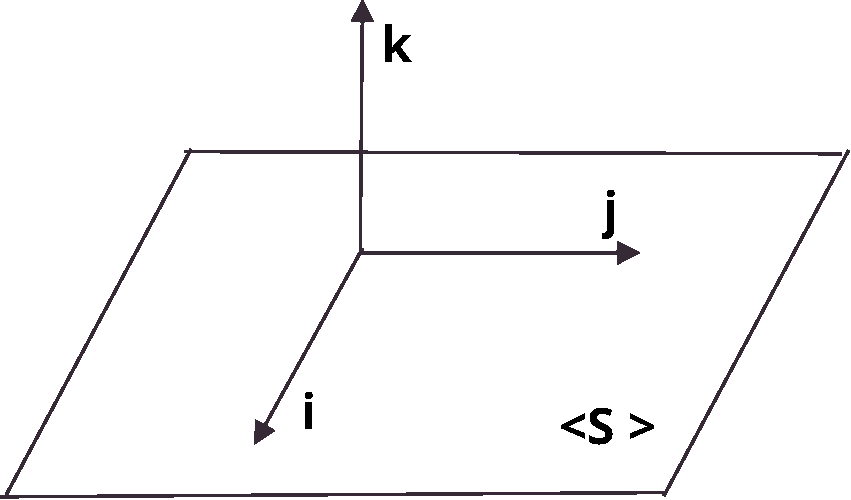
\includegraphics[width=6cm]{image/v3.pdf} $\widetilde{s} = \{i+j\}$ 
    \end{enumerate}
  \end{example}
  \begin{definition}
    Если $V=\langle S \rangle$, то $S$ называется порождающим множеством векторного простанства $V$. Говорят векторное пространство $V$ порождается множеством $S$. 
  \end{definition} 
  \begin{definition}
    Если $\exists$ конечное множество $S$, т.ч. $V=\langle S \rangle$, то $V$ называется конечномерным (конечнопорожденным), иначе бесконечномерным.
  \end{definition} 
  \begin{example1}
    $\R^n = \langle (1,0,...,0),...,(0,...,0,1) \rangle$ 
  \end{example1}
\begin{lemma} (Переформулировка ОЛЛЗ)
  Пусть векторное пространство $V$ пораждается $k$ векторами. Тогда любые $m>k$ векторов из $V$ - ЛЗ.
\end{lemma} 
\subsection{Базис}
$V$- конечномерное векторное простанство над $\R$ 
\begin{definition}\tab[-0.1cm]\textbf{1} 
  Система векторов $\{e_1,...,e_n\}\subseteq V$ называется бизисом векторного пространства $V$, если:
  \begin{enumerate}
    \item $\{e_1,...,e_n\}$ - ЛНЗ
    \item $V = \langle e_1,...,e_n \rangle$, т.е. $\forall x \in V, \tab[0.1cm] \exists \tab[0.1cm] x_1,...,x_n \in \R: x = x_1e_1+\cdots + x_ne_n$  
  \end{enumerate}
  Эти числа $x_1,...,x_n$ - называются координатами вектора $x$ в базисе $\{e_1,...,e_n\}$ 
\end{definition} 
\begin{definition}\tab[-0.1cm]\textbf{2} 
  Система векторов $\{e_1,...,e_n\} \subseteq V$ называется базисом векторного простанства $V$, если любой вектор $x \in V$ выражается через $\{e_1,...,e_n\}$ единственным образом.
\end{definition} 
  \begin{subtheorem}
    (\textbf{Опр 1}) $\Longleftrightarrow $ (\textbf{Опр 2})
  \end{subtheorem} 
  \begin{proof}
    По лемме \eqref{lem3}.
  \end{proof}
  \begin{theorem}
    Всякое конечномерное векторное пространство над $\R$ обладает базисом. Более того, из любого конечного порожденного множества можно выбрать базис.
  \end{theorem} 
  \begin{proof}
    Пусть $S$- какое-то порожденное множество векторного пространства $V$. \\
    Если $S$ - ЛНЗ, то $S$ - базис \\
    Если $S$ - ЛЗ, то по критерию о ЛЗ один из векторов $S_1$ множества $S$ линейно выражается через остальные. \\
    Тогда $S_1$ = $S\setminus\{s_1\}$ - конечное пораждащее множество. ч.т.д. \\
    Т.к. $S$ - конечное, это процесс прервется и мы получим ЛНЗ порожденную систему.
  \end{proof} 
  \begin{theorem}
    В любом базисе конечномерного векторного пространства $V$ над $\R$ одно и тоже число векторов.
  \end{theorem} 
  \begin{proof}
    Пусть есть два базиса $\{e_1,...,e_m\}$ и $\{f_1,...,f_m\}$ векторного пространства $V$. 
    Тогда каждый вектор $f_i$ выражается через $e_1,...,e_m$. \\
    По ОЛЛЗ: $\{f_1,...,f_m\}$ - ЛЗ $\Longrightarrow \{f_1,...,f_m\}$ - не базис $\Longrightarrow $ противоречие.  
  \end{proof} 
  \begin{definition}
    Число векторов в базисе конечномерного векторного пространства $V$, называется размерностью векторного простанства и обозначается: $dimV$ 
  \end{definition} 
  \begin{example} $\tab$ 
    \begin{enumerate}
      \item $dimV^2 = 2$
      \item $dim \R^n = n$   
    \end{enumerate}
  \end{example}
  \begin{remark}
    Если $V={0}$, то $dimV = 0$ (базис систоит из $\varnothing$ ) 
  \end{remark} 
   Пусть $V$- векторное пространство над $\R$, $dimV=n,\tab[0.1cm] S\subseteq V$ Любые $m>n$ векторов в $S$ - ЛЗ. (из ОЛЛЗ) \\
   $\Longrightarrow $ в $S \ \exists $ максимальная ЛНЗ подсистема (т.е. ничего нельзя добавить к этой подсистеме без нарушения ЛНЗ) 
  \begin{lemmanum} \label{lem6}
    Пусть $V$ - n-мерное векторное пространство над $\R,\tab[0.1cm] S\subseteq V$. Тогда максимальная ЛНЗ система векторов из $S$ образует базис в лин. оболочке $\langle S \rangle$  
  \end{lemmanum} 
  \begin{proof}
    Пусть $\{s_1,...,s_k\}$ максимальная (по включению) ЛНЗ система в $S$ $\Longrightarrow \forall s \in S \setminus \{s_1,...,s_k\}\Longrightarrow \{s,s_1,...,s_k\} - \text{ЛЗ.} $ \\
    По Лемме \eqref{lem2}. $\Longrightarrow s=\lambda_1s_1+\cdots+\lambda_ks_k$ \\
    Докажем, что $\{s_1,...,s_k\}$ базис в $\langle S \rangle$. 
    \begin{enumerate}
      \item ЛНЗ (очевидно)
      \item $\forall x \in \langle S \rangle\tab[-0.1cm]: x = x_1s_1+\cdots+x_ks_k$ 
    \end{enumerate}
    По определению линейной оболочки $x$ линейно выражается через вектора из $S$ \\
    А каждый вектор из $S$ линейно выражается через $\{s_1,...,s_k\}$ 
  \end{proof}
  \begin{theorem}
    Пусть $V$ конечномерное векторное пространство над $\R$, тогда:
    \begin{enumerate}
      \item Любая максимальная ЛНЗ система векторов из $V$ - базис $V$.
      \item Любую ЛНЗ систему векторов из $V$ можно дополнить до базиса векторного пространства $V$. 
    \end{enumerate}
  \end{theorem}  
  \begin{proof} $\tab$ 
    \begin{enumerate}
      \item По лемме \eqref{lem6}. $S=V$ 
      \item Пусть $S$ - ЛНЗ система векторов из $V$ 
    \end{enumerate}
    Если $V=\langle S \rangle$, тогда $S$- базис. \\
    Если $V \neq \langle S \rangle$ , то $\exists s_1 \in V \setminus \langle S \rangle$ \\
    $\Longrightarrow s_1$ линейно невыражается через $S$ $\Longrightarrow \text{(По лемме \ref{lem2}.) } S_1=S \cup \{s_1\}$ - ЛНЗ. \\
    $\Longrightarrow $ Если $V = \langle S \rangle$, то $S_1$ базис, иначе $\exists S_2 \in V \setminus \langle S_1 \rangle$, и т.д. \\
    Этот процесс прервется на конечном шаге, т.к. пространство $V$- конечное. (Если $dimV \neq n, \text{то} \not\exists$ ЛНЗ системы с числом векторов $> n$) 
  \end{proof} 
  \begin{consequense} 
    Пусть $V$ конечномерное векторное пространство над $\R$ 
    \begin{enumerate}
      \item Любой ненулевой вектор можно дополнить до базиса.
      \item Любые $n$ ЛНЗ вектора в $n$-мерном пространстве $V$ образуют базис.
    \end{enumerate}
  \end{consequense} 
  
  \section{Ранг}
  \subsection{Рангом системы векторного простанства}
  \begin{definition}
    Рангом системы векторного простанства $S\subseteq V$ называется $dim \langle S \rangle$  
  \end{definition} 
  $A$ - матрица $m \times n$ \\ $\\$
  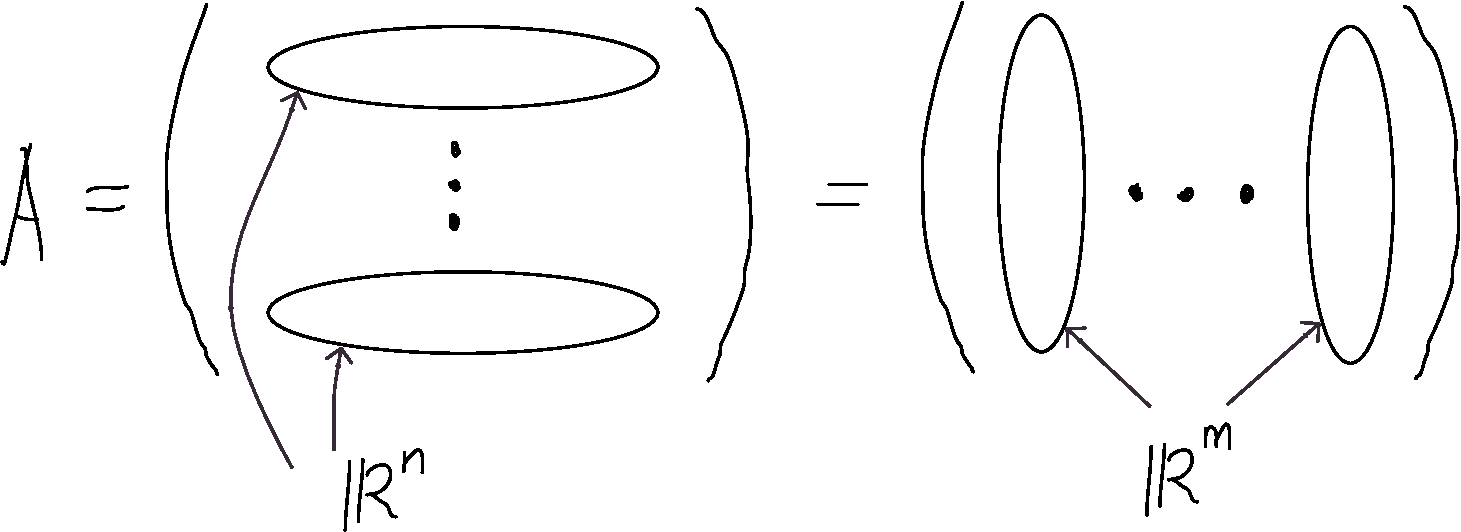
\includegraphics[width=15cm]{image/matr.pdf}
  \begin{definition}
    Рангом матрицы $A$ называется ранг системы ее строк, т.е. максимальное число ЛНЗ строк матрицы.
  \end{definition} 
  \subsection{Ранг матрицы}
  \begin{definition}
    Ранг системы $\{s_1,...,s_n\}$ - векторов называется $dim \langle s_1,...,s_n \rangle$.
  \end{definition} 
  \begin{definition}
    Рангом матрица $A \ m\times n$ называется ранг системы её строк. $$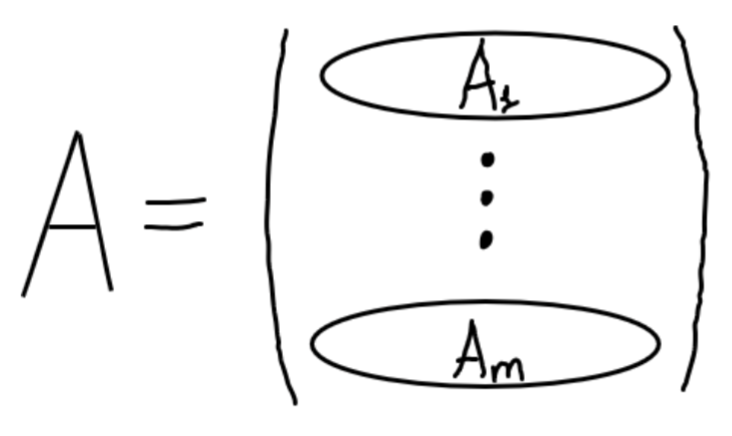
\includegraphics[width=4cm]{image/matr5.png}$$
  \end{definition} 
  \begin{definition}
    Две системы векторов $\{v_1,...,v_n\}$ $\{w_1,...,w_n\}$ называются эквивалентными, если каждый вектор $v_i$ линейно выражается через $\{w_1,...,w_n\}$, а $w_i$ через $\{v_1,...,v_n\}$. \\
    Это условная эквивалентность: $\langle v_1,...,v_n \rangle = \langle w_1,....,w_n \rangle$ 
  \end{definition} 
  \begin{subtheorem}
    При элементарных преобразованиях над строками, ранг матрицы $A$  не изменяется.
  \end{subtheorem} 
  \begin{proof} 
    $$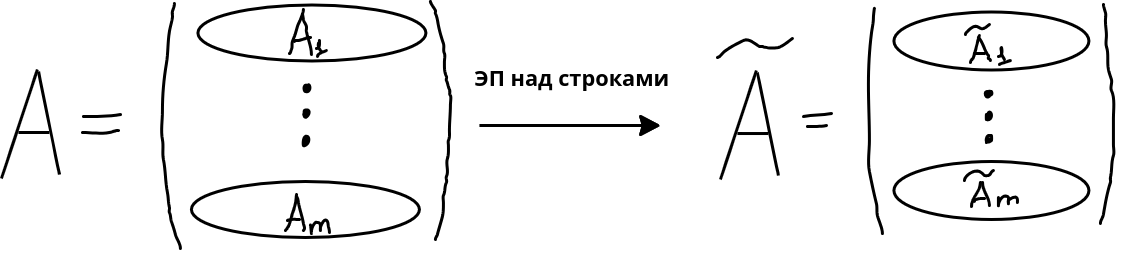
\includegraphics[width=12cm]{image/matr1.png}$$
    $$\langle A_1,...,A_m \rangle = \langle \widetilde{A_1},...,\widetilde{A_m} \rangle$$ \\
    т.е. система строк $A$ эквивалентна системы строк $\widetilde{A}$ $\Longrightarrow rkA = rk \widetilde{A}$. 
  \end{proof} 
  \begin{subtheorem}
    При элементарных преобразованиях над столбцами, ранг матрицы $A$  не изменяется.
  \end{subtheorem} 
  \textbf{Предложение 1.} \\
   Ранг матрицы $A$ равен числу ненулевых строк матрицы струпенчатого вида, к которому можно привести матрицу $A$ с помощью элементарных преобразований строк.
  \begin{proof}
    $A \overset{\text{ЭП строк}}{\longrightarrow } A_{\text{ст}} \Longrightarrow  rkA = rkA_{\text{ст}}$ \\
    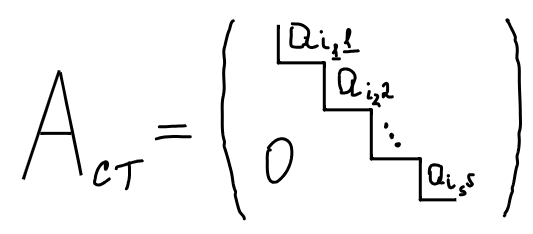
\includegraphics[width=5cm]{image/matr2.png}
    $a_{i_11},...,a_{i_ss}$ - лидеры строк в $A_{\text{ст}} \Longrightarrow a_{i_11} \neq 0,...,a_{i_ss} \neq 0$ \\
    Очевидно, что $rkA_{\text{ст}}\leq s$. Достаточно доказать, что ненулевые строки ЛНЗ. Рассмотрим ЛК: \\
    $\lambda_1(0,...,0,a_{i_11},\ast,...,\ast) + \lambda_2(0,...,0,a_{i_22},\ast,...,\ast) + \cdots + \lambda_s(0,...,0,a_{i_ss},\ast,...,\ast) = (0,...,0)$ \\
    $(0,...,0,\lambda_1 a_{i_11},...,\lambda_1a_{i_21} + \lambda_2a_{i_22},...) = (0,...,0) \Longrightarrow \lambda_1 \underbrace {a_{i_11}}_{\text{лидер}}= 0 \Longrightarrow \lambda_1 = 0$ \\
    $\lambda_1a_{i_21} + \lambda_2\underbrace {a_{i_22}}_{\text{лидер}} = 0 \Longrightarrow \lambda_2 = 0$ и т.д. \\
    Получаем, что $\lambda_1 = 0,...,\lambda_s = 0 \Longrightarrow$ это ЛК - ЛНЗ. 
  \end{proof} 
  \textbf{Предложение 2.} 
  Ранг системы столбцов не изменяется при элементарных преобразованиях над строками. 
  \begin{proof}  
    $A \overset{\text{ЭП строк}}{\longrightarrow } \widetilde{A}$. Пусть $A = (a_{ij}) = (\underbrace{A_1,...,A_n}_{\text{столбцы }A})$ 
    $\widetilde{A} = (\widetilde{a_{ij}}) = (\widetilde{A_1},...,\widetilde{A_n})$. 
    Докажем, что если для некоторого числа $\lambda_1,...,\lambda_n \in \R$ выполнено: $\lambda_{1}A_1 + \cdots + \lambda_nA_n = 0$, то для этих же чисел  $\lambda_1 \widetilde{A_1} + \cdots + \lambda_n \widetilde{A_n} = 0$ (Верно и обратное, т.к. ЭП обратимы, т.е. если для каких-то чисел $\lambda_i \in \R: \sum \lambda_i \widetilde{A_1} = 0$, то $\sum \lambda_i A_i = 0$). \\
    Дано: $\lambda_1A_1 + \cdots + \lambda_nA_n = \begin{pmatrix}
      0\\
      \vdots\\
      0\\
    \end{pmatrix}\Longrightarrow$ \\
    $ \begin{cases}
      \lambda_1a_{11} + \lambda_2a_{12} + \cdots + \lambda_na_{1n} = 0 \\
      \vdots \\
      \lambda_1a_{m1} + \lambda_2a_{m2} + \cdots + \lambda_na_{mn} = 0
    \end{cases}$ 
    $\Longrightarrow \lambda_1,...,\lambda_m - \text{решение ОСЛУ } AX=0$. \\ $\\$ 
    Т.к. при ЭП над уравнениями множество решений не меняется, поэтому $\lambda_1,...,\lambda_n$ - это решение ОСЛУ $\widetilde{A}X=0$
    $\Longrightarrow \lambda_1 \widetilde{A_1} + \cdots + \lambda_n \widetilde{A_n} = 0$ \\
    Отсюда получаем, что если $A_{i_1},...,A_{i_s}$ - максимальная ЛНЗ система столбцов в $A$, то $\widetilde{A_{i_1}},...,\widetilde{A_{i_s}}$ - максимальная ЛНЗ система столбцов в $\widetilde{A}$ $\Longrightarrow rk\{\widetilde{A_1},...,\widetilde{A_n}\} = rk\{A_1,...,A_n\}.$ 
  \end{proof} 
  \begin{definition}
    Пусть $A = (a_{ij})$ - матрица $m\times n $, тогда $B = (b_{ij}) \text{ матрица } n\times m$ называется транспонированной к матрице $A$, если $b_{ij} = a_{ji}$, где $i = \overline{1,m}; j = \overline{1,n}$ \\
    Обозначаем $B = A^T$  
  \end{definition} 
  \begin{example1}
    $$\begin{pmatrix}
      1&2&3\\
      4&5&6
    \end{pmatrix}^T
    = \begin{pmatrix}
      1&4\\
      2&5\\
      3&6
    \end{pmatrix}$$ 
  \end{example1}
  \begin{consequense} 
    Ранг системы строк матрицы $A$ (=рангу матрицы $A$) не изменяется при элементарных преобразованиях над столбцами. 
  \end{consequense} 
  \begin{proof}
    Предложение 2 применяем к $A^T$ 
  \end{proof} 
  \begin{theoremnum} 
    Ранг системы строк матрицы $A$ совпадает с рангом системы столбцов матрицы $A$.
  \end{theoremnum} 
  \begin{proof}
    Было доказанно, что ранг системы строк (столбцов) матрицы не изменяется при ЭП над строками и над столбцами. Приведем матрицу $A$ к ступенчатому виду с помощью ЭП над строками. $A_\text{ст}$ имеет вид:
    $$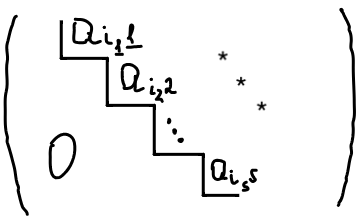
\includegraphics[width=4cm]{image/matr4.png}$$
    $$a_{i_11} \neq 0,...,a_{i_ss} \neq 0$$ 
    Используем $i_1$-столбец, вычитая этот столбец из оставшихся с подходящими коэфициентами, получаем:
    $$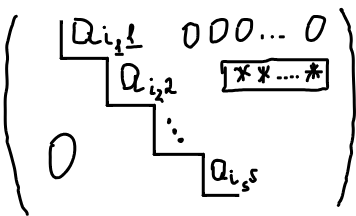
\includegraphics[width=4cm]{image/matr3.png}$$ 
    Далее используем $i_2$-столбец, обнуляем все элементы правее $a_{i_22}$. В итоге получаем: $$\begin{pmatrix}
      a_{i_1,1} && \null && 0\\
      \null && \ddots && \null\\
      0 && \null && a_{i_ss}
    \end{pmatrix}$$
    Очев, что у такой матрицы ранг системы строк = рангу системы столбцов.
  \end{proof} 
  \section{Возвращаемся к системе линейных уравнений}
  $\begin{cases}
    a_{11}x_1 + ... + a_{1n}x_n = b_1 \\ 
    a_{21}x_2 + ... + a_{2n}x_n = b_2 \\
    \vdots \\
    a_{m1}x_1 + ... + a_{mn}x_n = b_m
  \end{cases} (AX = B)$
  \begin{theorem} (Кронекера-Копелли)
    \begin{enumerate}
      \item (Критерий совместимости СЛУ) \\ CЛУ $AX = B$ совместна $\Longleftrightarrow rk(A|B) = rkA$ 
      \item (Критерий определенности СЛУ) \\ Совместная СЛУ $AX =B$ - определенна $\Longleftrightarrow rk(A|B) = rkA = n$ 
      \item (Критерий существования нетривиального решения у однородной СЛУ) \\ ОСЛУ $AX = 0$ имеет нетривиальное решение $\Longleftrightarrow rkA<n$ 
    \end{enumerate}
  \end{theorem}
  \textbf{Однородная СЛУ} \\  
  $\begin{cases}
    a_{11}x_1 + ... + a_{1n}x_n = 0 \\ 
    a_{21}x_1 + ... + a_{2n}x_n = 0 \\
    \vdots \\
    a_{m1}x_1 + ... + a_{mn}x_n = 0
  \end{cases} (AX = 0)$
  \begin{subtheorem}
    ОСЛУ всегда совместна, т.к. есть тривиальное решение.
  \end{subtheorem} 
  \begin{properties} $\tab$ 
    \begin{enumerate}
      \item Если $X^0$ = $\begin{pmatrix}
        x_1^0\\
        \vdots\\
        x_n^0 
      \end{pmatrix}$; \tab[0.3cm] $\widetilde{X^0}$ = $\begin{pmatrix}
        \widetilde{x_1^0}\\
        \vdots\\
        \widetilde{x_n^0} 
      \end{pmatrix}$ - решение ОСЛУ, \\ \tab[9cm] тогда $X^0 + \widetilde{X^0}$ = $\begin{pmatrix}
        X_1^0 + \widetilde{X_1^0} \\
        \vdots\\
        X_n^0 + \widetilde{X_n^0}
      \end{pmatrix}$
      \item Если $X^0$ = $\begin{pmatrix}
        x_1^0\\
        \vdots\\
        x_n^0 
      \end{pmatrix}$ - решение ОСЛУ $AX = 0$, то $\lambda X^0$ = $\begin{pmatrix}
        \lambda x_1^0\\
        \vdots\\
        \lambda x_n^0 
      \end{pmatrix}$ - решение.
    \end{enumerate}
  \end{properties}
  \begin{proof}
    Д/з
  \end{proof} 
  \begin{consequense}
    Множество всех решений ОСЛУ является векторным \\ подпространством в $\R^n$. Будем говорить, что это пространство над ОСЛУ.
  \end{consequense} 
  \begin{remark}
    Если $\exists$ решение ОСЛУ над $\R$, то $\exists$ бесконечно много решений.
  \end{remark} 
  \begin{theoremnum}
    Пространство решений ОСЛУ $AX = 0$ имеет базис из $n-r$ векторов, где $n$ - число неизвестных, а $r=rkA$.
  \end{theoremnum} 
  \subsection{Фундаментальная система решений}
  \begin{definition}
    Любой базис пространства решений ОСЛУ называется \\ Фундаментальной Системой Решений ОСЛУ (ФСР).
  \end{definition} 
  \begin{proof}
    (Теоремы 2.) \\ Решение СЛУ методом Гаусса: приводим её к ступенчатому виду (число ступенек $r=rkA$), главные неизвестные выражаем через свободные. 
    $$\begin{cases}
      x_1=c_{1,1}x_{r+1} + \cdots + c_{1,n-r}x_n \\
      \vdots\\
      x_r=c_{r,1}x_{r+1} + \cdots + c_{r,n-r}x_n
    \end{cases}$$ 
    Определим $n-r$ частных решений приравнивая одно из $x_1,...,x_n$ к 1, а остальные к 0. 
    $$F_1 = \begin{pmatrix}
      c_{11}\\
      \vdots\\
      c_{r1}\\
      \hline
      1\\
      0\\
      \vdots\\
      0
    \end{pmatrix}, \ \ F_2 = \begin{pmatrix}
      c_{12}\\
      \vdots\\
      c_{r2}\\
      \hline
      0\\
      1\\
      \vdots\\
      0
    \end{pmatrix} \ ,..., \ F_{n-r} = \begin{pmatrix}
      c_{1,{n-r}}\\
      \vdots\\
      c_{r,{n-r}}\\
      \hline
      0\\
      0\\
      \vdots\\
      1
    \end{pmatrix}$$  
    Докажем, что $F_1,...,F_{n-r}$ - базис пространства ренений ОСЛУ 
    \begin{enumerate}
      \item $F_1,...,F_{n-r}$ - ЛНЗ? \\
      Рассмотрим ЛК $\lambda_1F_1 + \cdots + \lambda_{n-r}F_{n-r} = \begin{pmatrix}
        0 \\ \vdots \\ 0
      \end{pmatrix} \\ \Longrightarrow \begin{pmatrix}
        \ast \\ \vdots \\ \ast \\ \hline \lambda_1 \\ \vdots \\ \lambda_{n-r}
      \end{pmatrix} = \begin{pmatrix}
        0 \\ \vdots \\ 0
      \end{pmatrix} \Longrightarrow \lambda_1 = 0,...,\lambda_{n-r}=0$ 
      \item Надо доказать, что любое решение выражено через $F_1,...,F_{n-r}$ \\ $\\$ 
      $X^0 = \begin{pmatrix}
        c_{11} \\ \vdots \\ c_{r1} \\ \hline \mu_{r+1} \\ \vdots \\ \mu_n
      \end{pmatrix} = \mu_{r+1}F_1 + \cdots + \mu_nF_{n-r}$ 
    \end{enumerate}
  \end{proof}
  \newpage
  \begin{example1} Найти ФСР ОСЛУ \end{example1} 
  $\begin{cases}
    x_1 + x_2 + 3x_3+5x_4-x_5 = 0\\
    x_1 + 2x_2 + x_3 + x_4 + x_5 = 0
  \end{cases}$ 
  $$\begin{pmatrix}
    1 & 1 & 3 & 5 & -1 \\
    1 & 2 & 1 & 1 & 1
  \end{pmatrix}\rightarrow 
  \begin{pmatrix}
    1 & 1 & 3 & 5 & -1 \\
    0 & 1 & -2 & -4 & 2 
  \end{pmatrix} \rightarrow
  \begin{pmatrix}
    1 & 0 & 5 & 9 & -3 \\
    0 & 1 & -2 & -4 & 2
  \end{pmatrix}$$
  где $x_1, x_2$ - главные, $x_3, x_4, x_5$ - свободные \\ $\\$ 
  $\begin{cases}
    x_1 = -5x_3 - 9x_4 +3x_5 \\
    x_2 = 2x_3+4x_4-2x_5
  \end{cases}$ $x_3, x_4, x_5 \in \R$ - произвольные 
  $$F_1 = \begin{pmatrix}
    -5 \\ 2 \\ \hline 1 \\ 0 \\ 0
  \end{pmatrix}, \tab[0.5cm] F_2 = \begin{pmatrix}
    -9 \\ 4 \\ \hline 0 \\ 1 \\ 0
  \end{pmatrix}, \tab[0.5cm] F_3 = \begin{pmatrix}
    3 \\ -3 \\ \hline 0 \\ 0 \\ 1
  \end{pmatrix} \tab[0.1cm] \text{ - три частных решения ОСЛУ}$$ 
  Проверим, что $\{F_1,F_2, F_3\}$- базис пространства решений ОСЛУ \\ $\\$ 
  $\begin{pmatrix}
    * \\ * \\ \hline \lambda_1 \\ \lambda_2 \\ \lambda_3
  \end{pmatrix} = 
  \lambda_1F_1 + \lambda_2F_2 + \lambda_3F_3 = \begin{pmatrix}
    0 \\ 0 \\ 0 \\ 0 \\ 0
  \end{pmatrix} \Longrightarrow \lambda_{1,2,3} = 0 \Longrightarrow F_1, F_2, F_3$ - ЛНЗ. \\ $\\$ 
  Проверим, что $\{F_1,F_2, F_3\}$ порождает пространство решений. Возьмем произвольные числа $\mu_3, \mu_4, \mu_5$ и приравняем $x_3 = \mu_3, x_4 = \mu_4, x_5 = \mu_5$  
  $$\begin{pmatrix}
    x_1 \\ x_2 \\ \hline x_3 \\ x_4 \\ x_5
  \end{pmatrix} = \begin{pmatrix}
    -5\mu_3-9\mu_4+3\mu_5 \\ 2\mu_3 + 4\mu_4-2\mu_5 \\ \hline \mu_3 \\ \mu_4 \\ \mu_5
  \end{pmatrix} = \mu_3 \begin{pmatrix}
    -5 \\ 2 \\ \hline 1 \\ 0 \\ 0
  \end{pmatrix} + \mu_4 \begin{pmatrix}
    -9 \\ 4 \\ \hline 0 \\ 1 \\ 0
  \end{pmatrix} + \mu_5 \begin{pmatrix}
    3 \\ -2 \\ \hline 0 \\ 1 \\ 1 
  \end{pmatrix}$$ 
  Такой базис называется нормальный ФСР. 
  \subsection{Неоднородная СЛУ}
  $\begin{cases}
    a_{11}x_1 + ... + a_{1n}x_n = b_1 \\ 
    a_{21}x_2 + ... + a_{2n}x_n = b_2 \\
    \vdots \\
    a_{m1}x_1 + ... + a_{mn}x_n = b_m
  \end{cases} (AX=B)$ \\ $\\$ 
  Рассмотрим соответствующую ОСЛУ \\ $\\$ 
  $\begin{cases}
    a_{11}x_1 + ... + a_{1n}x_n = 0 \\ 
    a_{21}x_2 + ... + a_{2n}x_n = 0 \\
    \vdots \\
    a_{m1}x_1 + ... + a_{mn}x_n = 0
  \end{cases} (AX=0)$ 
  \begin{theorem}
    Пусть СЛУ $AX=B$ - совместна. $X_0$ - произвольное частное решение. Тогда множество $M$ всех решений неоднородной СЛУ: $AX=B$ равно сумме частного решения $X_0$ и множество $M_{\text{одн}}$ всех решений соответствующей осднородной СЛУ: $AX=0$ 
    $$M = X_0 + M_{\text{одн}} = \{X_0 + Y | Y \in M_{\text{одн}}\}$$ 
  \end{theorem}
  \begin{proof}
    $X_0 + M_{\text{одн}} \subseteq M$ \\
    Рассмотрим произвольное решение ОСЛУ. $Y \in M_{\text{одн}}$ \\ $\\$ 
    Пусть $X_0 = \begin{pmatrix}
      x_1^0 \\ \vdots \\ x_n^0
    \end{pmatrix}, \tab[0.2cm] Y = \begin{pmatrix}
      y_1 \\ \vdots \\ y_n
    \end{pmatrix}$ \\
    \tab[1.8cm]Докажем, что $X_0 + Y = \begin{pmatrix}
      x_1^0 + y_1 \\ \vdots \\ x_n^0 + y_n
    \end{pmatrix}$ - решение СЛУ, т.е. $X_0 + Y \in M$ 
    $$AX=B a_{i1}x_1 + \cdots + a_{in} = b_i$$
    $$AX=0 a_{i1}x_1 + \cdots + a_{in} = 0$$
    где $i = \overline{1,n}$. \\
    Проверим, что $X_0 + Y \in M$ 
    $$a_{i1}(x_1^0 + y_1) + \cdots + a_{in}(x_{in} + y_n) = b_i$$
    $$(\underbrace{a_{i1}x_1^0 + \cdots + a_{in}x_{in}}_{b_i (\text{т.к. } X_0 \in M)}) + (\underbrace{a_{i1}y_1 + \cdots + a_{in}y_n}_{0 (\text{т.к. } Y \in M_{\text{одн}})}) = b_i$$  
    Обратное утверждение:
    $M \subseteq X_0 + M_{\text{одн}}$ \\
    Рассмотрим произвольное решение $Z = \begin{pmatrix}
      z_1 \\ \vdots \\ z_n 
    \end{pmatrix}$ - неоднородная СЛУ. \\
    Докажем, что $Z - X_0 = \begin{pmatrix}
      z_1 - x_1^0 \\ \vdots \\ z_n - x_n^0
    \end{pmatrix}
    $ - решение однородной СЛУ. \\
    Проверяем
    $$a_{i1}(z_1 - x_1^0) + \cdots + a_{in}(z_n - x_n^0) = 0$$ 
    $$(\underbrace{a_{i1}z_1 + \cdots + a_{in}z_n}_{b_i (\text{т.к. } Z \in M)}) - (\underbrace{a_{i1}x_1^0 + \cdots + a_{in}x_n^0}_{b_i (\text{т.к. } X_0 \in M)}) = 0$$ 
  \end{proof}  
  \begin{remark} $\\$ 
    Общее решение ОСЛУ имеет вид вид: $$X = \mu_1F_1 + \cdots + \mu_sF_s$$где $F_1,...,F_s$ - ФСР ОСЛУ, $s = n - rkA$  \\
    Общее решение неоднородной СЛУ: $$X = X_0 + \mu_1F_1 + \cdots + \mu_sF_s$$ $X_0$ - частное решение неоднородной СЛУ
  \end{remark} 
  \section{Операции над матрицами}
  $Mat_{m \times n}(\R)$ - множество всех матриц размера $m \times n$ с коэфициентами из $\R$ \\
  $A, B \in Mat_{m \times n}(\R), A=(a_{ij}), B=(b_{ij})$ 
  \begin{enumerate}
    \item Сложение матриц \\
    Суммой матриц $A$ и $B$ называется матрица $C=(c_{ij})$ размера $m \times n$, у которой $c_{ij} = a_{ij} + b_{ij}$. Обозначается: $C = A + B$
    \item Умножение матриц на число $\lambda \in \R$ \\ Произведение матрицы $A=(a_{ij})$ на $\lambda$ называется матрица $C=(c_{ij})$ размера $m \times n$, у которой $c_{ij} = \lambda a_{ij}$. Обозначается: $C = \lambda A$
    \begin{subtheorem}
      Множество $Mat_{m \times n}(\R)$ относительно этих операций сложения и умножения на число, образует векторное пространство над $\R$. 
    \end{subtheorem} 
    \begin{proof}
      $A,\tab [0.2cm]B \in Mat_{m \times n}(\R) \Longrightarrow A+B, \tab [0.2cm]\lambda A \in Mat_{m \times n}(\R)$ \\
      Надо проверить 8 аксиом
      \begin{itemize}
        \item[1)] коммутативность \\
        $C = A + B \tab[0.5cm] c_{ij} = a_{ij} + b_{ij}$ \\
        $\widetilde{C} = B + A \tab[0.5cm] \widetilde{c_{ij}} = b_{ij} + a_{ij}$ \\
        т.к. сложение вещественных чисел из $\R$ - коммутативно, то $c_{ij} = \widetilde{c_{ij}} \Longrightarrow C = \widetilde{C}$ \\
        $\Longrightarrow A + B = B + A$
        \begin{lalala} Аналогично доказать 2), 5)-8)\end{lalala}
        \item[3)] $\exists 0 \in Mat_{m \times n}(\R)$
        $\forall A \in Mat_{m \times n}(\R): 0 + A = A$ \\
        В качестве 0 берем нулевую матрицу размера $m \times n$
        \item[4)] $\forall A \in Mat_{m \times n}(\R) \ \exists B \in Mat_{m \times n}(\R): A+B=0$ \\В качестве $B$ берем $b_{ij} = -a_{ij}$ 
      \end{itemize}
    \end{proof} 
    \begin{lalala}
      $dimM_{m \times n} = m \cdot n$ 
    \end{lalala}
    \begin{proof}
      Достаточно указать базис \\ 
      $\{E_{st}\}$, $s = \overline{1,m}, \ t = \overline{1,n}$ \\
      $E_{st} = (a_{ij})$, $a_{ij} = \begin{cases}
        1, \ i=s, \ j=t \\ 0 \text{, иначе}
      \end{cases}$
      \begin{lalala}
        Проверить, что это базис.
      \end{lalala}  
    \end{proof} 
    \begin{definition}
      Матрица $E_{st}$ называется матричной единицей. Базис из всех матричных единиц называется стандартным базисом в пространстве $Mat_{m \times n}(\R)$. $A = \sum a_{st} E_{st}$ 
    \end{definition} 
    \item Умножение матриц \\
    $A \in Mat_{m \times k}(\R), \tab[0.2cm]B \in Mat_{k \times n}(\R)$ \\
    Произведение матрицы $A$ на матрицу $B$ называется матрица $C$ размера $m \times n$, у которой $c_{ij} = \sum \limits_{s=1}^{k}a_{is}b_{sj}$. Обозначаем $C = AB$.
    \begin{properties1}
      Произведение матриц не коммутативно.
    \end{properties1}
    \begin{example1}
      $$A = \begin{pmatrix}
        1 & 0 \\ 0 & 0
      \end{pmatrix}, \tab[0.3cm] B = \begin{pmatrix}
        0 & 1 \\ 0 & 0
      \end{pmatrix}$$
      $$AB = \begin{pmatrix}
        0 & 1 \\ 0 & 0
      \end{pmatrix}, \tab[0.3cm] BA = \begin{pmatrix}
        0 & 0 \\ 0 & 0
      \end{pmatrix} \Longrightarrow AB \neq BA$$ 
    \end{example1}
    \begin{remark} $\\ \\$
      $\begin{cases}
        a_{11}x_1 + \cdots + a_{1n}x_n = b_1 \\
        \vdots \\
        a_{m1}x_1 + \cdots + a_{mn}x_n = b_n
      \end{cases} \Longleftrightarrow \begin{pmatrix}
        a_{11} & \cdots & a_{1n} \\
        \vdots & \null & \vdots \\
        a_{m1} & \cdots & a_{mn}
      \end{pmatrix} \begin{pmatrix}
        x_1 \\ \vdots \\ x_n
      \end{pmatrix} = \begin{pmatrix}
        b_1 \\ \vdots \\ b_m
      \end{pmatrix}$
    \end{remark} 
  \end{enumerate}
  \begin{example}\end{example}
    \begin{enumerate}
      \item Проекция \\
      $\phi: V^3 \to V^2, \phi: x_1i+x_2j+x_3k \to x_1i+x_2j$ 
      $$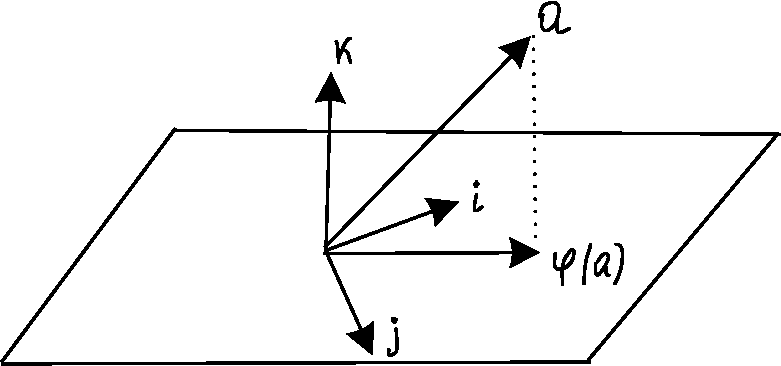
\includegraphics[width=6cm]{image/projection.pdf}$$
      \item Поворот\\
      $\phi: V^2 \to V^2$ Поворот на угол $\alpha$ вокруг точки $O$ 
      $$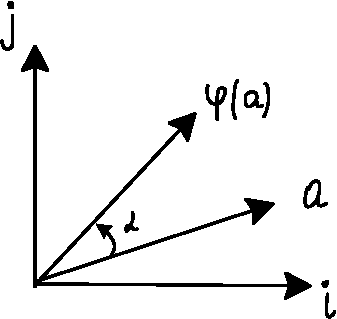
\includegraphics[width=3.5cm]{image/turn.pdf}$$
    \end{enumerate}
    
  \section{Линейные отображения}
  \subsection{Изоморфизм}
  
  $V, W$- векторные пространства над $\R$ 
  \begin{definition}
    Отображение $\phi: V \to W$ называется изоморфизмом векторных пространств, если:
    \begin{enumerate}
      \item $\forall a, b \in V: \ \phi(a+b) = \phi(a) + \phi(b)$
      \item $\forall \lambda \in \R \ \forall a \in V: \ \phi(\lambda a) = \lambda \phi(a)$
      \item $\phi$ является биекцией. 
    \end{enumerate}
    При этом $V, W$ называется изоморфными. Обозначается $V \cong W$ 
  \end{definition} 
  \begin{subtheorem}
    Любое векторное  пространство над $\R$ размерности $n$ изоморфно $\R^n$. 
  \end{subtheorem} 
  \begin{proof}
    Фиксируем базис $\{e_1,...,e_n\}$ - в $V$.
    \begin{enumerate}
      \item $\forall x \in V$ однозначно раскладывается по базису $x = \sum \limits_{i=1}^{n} x_ie_i$. 
    Зададим отображение  $\phi: V \to \R^n$ по правилу:
    $$\phi: x = x_1e_1 + \cdots + x_ne_n \to (x_1,...,x_n)$$
    Т.к. координаты вектора определены однозначно, то $\phi$ инъективно, сюрьективность очевидна $\Longrightarrow $ $\phi$ - биекция.
    \item $\forall x,y \in V$
    $$x = \sum \limits_{i=1}^{n} x_ie_i \tab[0.5cm] y = \sum \limits_{i=1}^{n} y_ie_i \tab[0.5cm]
    x + y = \sum \limits_{i=1}^{n} (x_i + y_i)e_i$$ 
    $$\phi(x+y) = (x_1 + y_1,...,x_n+y_n) = (x_1,...,x_n) + (y_1,...,y_n) = \phi(x) + \phi(y)$$ 
    \item $\forall \lambda \in \R \tab[0.1cm] \forall x \in V$
    $$\phi(\lambda x) = \phi(\sum \limits_{i=1}^{n} \lambda x_ie_i) = (\lambda x_1,....,\lambda x_n) = \lambda (x_1,...,x_n) = \lambda \phi(x)$$  
    \end{enumerate}
  \end{proof} 

  \begin{example}\end{example}
  \begin{enumerate}
    \item $V^2 \cong \R^2 \\ V^3 \cong \R^3$ 
    \item $M_{m \times n}(\R) \cong \R^{mn}$
  \end{enumerate}
  \begin{lalala}
    $V \cong W \Longleftrightarrow dimV = dimW; \tab[0.2cm] V,W - $ конечномерные пространства над $\R$.  
  \end{lalala}
  \subsection{Линейные отображение и матрицы}
  \begin{definition}
    Отображение $\phi: V \to W$ называется линейным, если
    \begin{enumerate}
      \item $\forall a,b \in V \tab[0.3cm] \phi(a+b) = \phi(a) + \phi(b)$
      \item $\forall \lambda \in \R, \forall a \in V \tab[0.3cm] \phi(\lambda a) = \lambda \phi(a)$  
    \end{enumerate}
    
  \end{definition} 
  \begin{subtheorem}
    $V,W$- векторные пространства над $\R$. \\
      Если $\{e_1,...,e_n\}$ - базис $V$, ($w_1,...,w_n$) - набор векторов из $W$. \\Тогда $\exists$! линейное отображение $\phi: V \to W$, которое $\phi: e_i \to w_i \tab[0.3cm]\forall i = \overline{1,n}$.
  \end{subtheorem} 

  \begin{proof} \tab
    \begin{enumerate}
      \item Пусть $\phi: V \to W$ - линейное отображение такое, что \\$\phi(e_i) = w_i \tab[0.2cm] \forall i = \overline{1,n}$. Тогда образ вектора $x$ определяется однозначно по формуле: $$\phi(x) = \phi(x_1e_1 + \cdots + x_ne_n) = x_1 \phi(e_1) + \cdots + x_n \phi(e_n) = x_1 w_1 + \cdots + x_n w_n$$ где $x=x_1e_1 + \cdots + x_ne_n$ \\
      $\Longrightarrow$ линейное отображение определяется однозначно.
      \item Докажем, что $\exists$ линейное отображение, которое переводит $e_i$ в $w_i$. Отображение зададим формулой: $$\phi: x = x_1e_1 + \cdots + x_ne_n \to x_1w_1 + \cdots + x_nw_n$$
      $$\phi(a+b) = \phi((a_1+b_1)e_1 + \cdots + (a_n + b_n)e_n) = (a_1+b_1)w_1 + \cdots + (a_n + b_n)w_n$$
      $$\phi(a) + \phi(b) = \phi(a_1e_1 + \cdots a_ne_n) + \phi(b_1e_1 + \cdots b_ne_n) = $$ $$= a_1w_1 + \cdots + a_nw_n + b_1w_1 + \cdots + b_nw_n = w_1(a_1 + b_1) + \cdots + w_n(a_n + b_n)$$
      $\Longrightarrow \phi(a+b) = \phi(a) + \phi(b)$\\
      Проверить, что $\phi(\lambda a) = \lambda \phi(a)$ - ДЗ
    \end{enumerate}
  \end{proof} 
  Пусть $\phi: V \to W$ - линейное отображение $V$- $n$-мерное, $W - m$-мерное пространство.  \\
  Фиксируем базис 
  $\mathcal{E}  = \{e_1,...,e_n\}$ - базис в $V$; $\mathcal{F}  = \{f_1,...,f_m\}$ - базис в $W$
  $$\phi(e_1) = w_1 = a_{11}f_1 + \cdots + a_{m1}f_m$$ $$\vdots$$
  $$\phi(e_n) = w_n = a_{1n}f_1 + \cdots + a_{mn}f_m$$

  \begin{definition}
    Матрица $A$ размера $m \times n$,  составленая из столбцов координат образов векторов $e_i$ в образе $\mathcal{F}$, называется матрицей линейного отображения в базисах $\mathcal{E} $ и $\mathcal{F}$  
  \end{definition} 
  $$A = \begin{pmatrix}
    a_{11} & \cdots & a_{1n} \\
    \vdots & \null & \vdots \\
    \undermat{\phi(e_1)}{a_{m1}}  & \cdots & \undermat{\phi(e_n)}{a_{mn}} 
  \end{pmatrix}$$  
  \vspace{0.3cm}
  \begin{subtheorem}
    Пусть $\mathcal{E}  = \{e_1,...,e_n\}$ - базис в $V$ над $\R$ ; $\mathcal{F}  = \{f_1,...,f_n\}$ - базис в $W$ над $\R$. Тогда:
    \begin{itemize}
      \item Каждому линейному отображению $\phi: V \to W$ однозначно соответствуют матрица размера $m \times n$ этого линейного отображения в базисах $\mathcal{E}, \mathcal{F}$
      \item Любой матрицы $A$ размера $m \times n$ однозначно соответствует линейное отображение $\phi: V \to W$, для которого $A$ - матрица этого линейного отображения в $\mathcal{E}, \mathcal{F}$.
    \end{itemize}
  \end{subtheorem} 

  \subsection{Операции над линейными отображениями}
  Пусть $V,W$ - векторные пространства над $\R$
  \begin{itemize}
    \item[1)] Сложение линейных отображений. $$\phi_1:V \to W \tab[0.4cm] \phi_2:V \to W \text{ - два линейных отображения}$$  
    Зададим отображение по правилу $$(\phi_1 + \phi_2)(x) = \phi_1(x) + \phi_2(x) \tab[0.3cm] \forall x \in V$$ 
    \begin{subtheorem}
      Отображение $\phi_1 + \phi_2: V \to W$ является линейным отображением.
      \begin{proof}
        $\forall a,b \in V$: $$(\phi_1 + \phi_2)(a+b) = \phi_1(a+b) + \phi_2(a+b) = $$ 
        $$ = \phi_1(a) + \phi_1(b) + \phi_2(a) + \phi_2(b) = (\phi_1 + \phi_2)(a) + (\phi_1 + \phi_2)(b)$$ 
        Аналогично для $(\phi_1 + \phi_2)(\lambda a) = \lambda (\phi_1 + \phi_2)(a)$ 
      \end{proof} 
    \end{subtheorem} 

    Фиксируем базисы $\mathcal{E}  = \{e_1,...,e_n\}$ - в $V$ и $\mathcal{F}  = \{f_1,...,f_n\}$ - в $W$

    $A_1$ - матрица линейного отображения $\phi_1$ относильно $\mathcal{E}$ и $\mathcal{F}$. \\
    $A_2$ - матрица линейного отображения $\phi_2$ относильно $\mathcal{E}$ и $\mathcal{F}$. \\
    $B$ - матрица линейного отображения $\phi_1+\phi_2$ относильно $\mathcal{E}$ и $\mathcal{F}$.
    \begin{subtheorem}
      $B=A_1 + A_2$ 
    \end{subtheorem} 
    \begin{proof}
      Размеры совпадают
      $$\phi_1(e_i) = a_{1i}f_1 + \cdots + a_{mi}f_m$$
      $$\phi_2(e_i) = \widetilde{a_{1i}} f_1 + \cdots + \widetilde{a_{mi}} f_m$$ 
      $$(\phi_1 + \phi_2)(e_i) = b_{1i}f_1 + \cdots + b_{mi}f_m$$ 
      $$(\phi_1 + \phi_2)(e_i) = \phi_1(e_i) + \phi_2(e_i) = (a_{1i}f_1 + \cdots + a_{mi}f_m) + (\widetilde{a_{1i}} f_1 + \cdots + \widetilde{a_{mi}} f_m) =$$ $$= (a_{1i} + \widetilde{a_{1i}})f_1 + \cdots + (a_{mi} + \widetilde{a_{mi}})f_m$$
      Т.к. разложение по базису единственное, то
      $$b_{1i} = a_{1i} + \widetilde{a_{1i}} ,..., b_{mi} = a_{mi} + \widetilde{a_{mi}} \Longrightarrow b_{ij} = a_{ij} + \widetilde{a_{ij}} \Longrightarrow B = A_1 + A_2$$ 
    \end{proof} 
    \item[2)] Умножение линейного отображение на число. \\
    $\phi: V \to W$ - линейное отображение, $\mu \in \R$ - произвольное число. \\
    Зададим отображение по правилу: $(\mu \phi)(x) = \mu \phi(x)$ $\tab[0.2cm] \forall x \in V$ 
    \begin{subtheorem}
      Отображение $\mu \phi: V \to W$ является линейным (Упражнение) 
    \end{subtheorem}
    \begin{proof}
      Аналогично.
    \end{proof} 
    Пусть $\mathcal{E}  = \{e_1,...,e_n\}$ - базис в $V$ и $\mathcal{F}  = \{f_1,...,f_n\}$ - базис в $W$. \\
    $A$ - матрица линейного отображения $\phi$ относильно $\mathcal{E}$ и $\mathcal{F}$. \\
    $B$ - матрица линейного отображения $\mu\phi$ относильно $\mathcal{E}$ и $\mathcal{F}$.
    \begin{subtheorem}
      $B=\mu A$ 
    \end{subtheorem} 
    \begin{proof}
      Видимо дз(
    \end{proof} 
    \item[3)] Композиция (произведение) линейных отображений. \\
    Пусть $V, W, U$ - векторные простанства над $\R$
    $$\phi: V \to W \tab[0.5cm] \psi: W \to U$$
    $$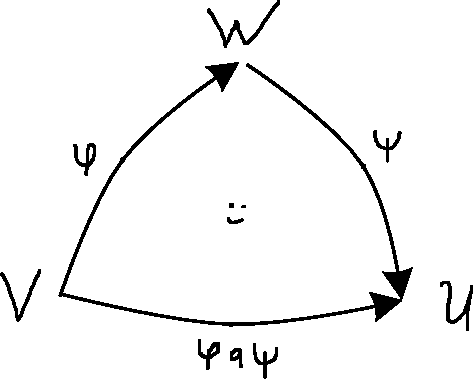
\includegraphics[width=5.5cm]{image/composition1.pdf}$$
    Зададим отображение по правилу: 
    $$(\psi \circ \phi)(x) = \psi(\phi(x)) \tab[0.3cm] \forall x \in V$$   
    \begin{subtheorem}
      Отображение $\psi \circ \phi: V \to U$ является линейным.
    \end{subtheorem} 
    \begin{proof}
      $\forall a, b \in V$
      \begin{enumerate}
        \item $(\psi \circ \phi)(a+b) = \psi(\phi(a+b)) = \psi(\phi(a)+\phi(b)) = \psi(\phi(a))+\psi(\phi(b))$ 
        \item Аналогично для $(\psi \circ \phi)(\lambda a) = \lambda(\psi \circ \phi)(a)$ 
      \end{enumerate}
    \end{proof} 

    Фиксируем базис: \tab[0.3cm]$\mathcal{E} = \{e_1,...,e_n\}$ - базис в $V$ \\
    \tab[4.3cm]$\mathcal{F} = \{f_1,...,f_m\}$ - базис в $W$ \\
    \tab[4.3cm]$\mathcal{G} = \{g_1,...,g_k\}$ - базис в $U$ \\
    $\underset{m \times n}{A}$ - матрица линейного отображения $\phi$ относительно $\mathcal{E}, \mathcal{F}$. \\
    $\underset{k \times m}{B}$ - матрица линейного отображения $\psi$ относительно $\mathcal{F}, \mathcal{G}$. \\
    $\underset{k \times n}{C}$ - матрица линейного отображения $\phi$ относительно $\mathcal{E}, \mathcal{G}$.
    \begin{subtheorem}
      $C = B \cdot A$ 
    \end{subtheorem} 
    \begin{proof}
      $$\phi(e_i) = \sum \limits_{s=1}^ka_{si}f_s; \tab[1cm]\psi(f_s) = \sum \limits_{t=1}^kb_{ts}g_t$$
      По определению матрицы линейного отображения:
      $$(\psi \circ \phi)(e_i) = \sum \limits_{l=1}^kc_{li}g_l \tab[0.3cm](\ast)$$ 
      По определению композиции:
      $$(\psi \circ \phi)(e_i) = \psi(\phi(e_i)) = \psi(\sum \limits_{s=1}^ma_{si}f_s) = \sum \limits_{s=1}^ma_{si}\psi(f_s) =\tab[4cm]$$ $$\tab[7cm]= \sum \limits_{s=1}^ma_{si}(\sum \limits_{t=1}^kb_{ts}g_t) = \sum \limits_{t=1}^k(\sum \limits_{s=1}^mb_{ts}a_{si})g_m \tab[0.3cm](\star)$$
      $\Longrightarrow $$(\ast) = (\star)$.\\
      Т.к. координаты определены однозначно $\Rightarrow c_t = \sum \limits_{s=1}^mb_{ts}a_{si} \Rightarrow C =B \cdot C$  
    \end{proof} 
  \end{itemize}
  \subsection{Свойства операций над матрицами}
  Предположим, что все размеры матриц согласованы. 
  \begin{enumerate}
    \item $M_{m \times n}(\R)$ - векторное пространство над $\R$
    \item Ассоциативность  $A(BC) = (AB)C$ 
    \begin{proof}
    $\underset{m \times k}{A} , \tab[0.1cm]\underset{k \times n}{B} , \tab[0.1cm]\underset{n \times l}{C}$ $\vspace{0.1cm}$

    Пусть $\underset{m \times l}{D} = A(BC), \tab[0.1cm]\underset{m \times l}{\widetilde{D}} = (AB)C$. 
    Надо проверить, что $\forall i,j: [D]_{ij} = [\widetilde{D}]_{ij}$. 
    $$[D]_{ij} = [A(BC)]_{ij} = \sum \limits_{s=1}^k[A]_{is} \cdot [BC]_{si} = \sum \limits_{s=1}^k[A]_{is}(\sum \limits_{t=1}^n[B]_{st} \cdot [C]_{ti}) = $$ $$  = \sum \limits_{s=1}^k \sum \limits_{t=1}^n[A]_{ij}([B]_{st} \cdot [C]_{ti})$$ 
    $$[\widetilde{D}]_{ij} = [(AB)C]_{ij} = \sum \limits_{t=1}^n[AB]_{it}[C]_{tj} = \sum \limits_{t=1}^n (\sum \limits_{s=1}^k[A]_{is} \cdot [B]_{st})[C]_{tj} = $$
    $$ = \sum \limits_{t=1}^n \sum \limits_{s=1}^k ([A]_{is} \cdot [B]_{st}) \cdot [C]_{tj}$$  
    По свойствам операций над $\R$, результаты преобразований равны.
    \end{proof} 
    \item $A(B+C) = AB + AC$
    \item $(B + C)A = BA + CA$  
    \item $\lambda(AB) = (\lambda A) B = A(\lambda B); \tab[0.3cm]\forall \lambda \in \R$ 
    \item $\forall A \in M_{m \times m}(\R)$, $\exists$  единичная матрица $E \in M_{m \times m}(\R)$ : 
    $EA = A$  
    \item $\forall A \in M_{m \times n}(\R)$ : $0 \cdot A = 0$ 
    \item Нет коммутативности: $AB \neq BA$ даже если размеры согласованы 
    \begin{proof}
      Свойства 3. - 7. упражнение)
    \end{proof} 
  \end{enumerate}
  \subsection{Свойства операции транспонирования}
  \begin{enumerate}
    \item $(A^T)^T = A$
    \item $(\lambda A)^T = \lambda A^T$
    \item $(A+B)^T + A^T + B^T$
    \item $(AB)^T = B^TA^T$   
    \begin{proof}
      4. $\underset{m \times k}{A}, \underset{k \times n}{B} \Longrightarrow \underset{n \times k}{B^T}, \underset{k \times m}{A^T}$ (размеры совпадают) \\
      Проверим $D = (AB)^T \text{ и } \widetilde{D} = B^TA^T$ равны.
      $$[D]_{ij} = [(AB)^T]_{ij} = [(AB)]_{ji} = \sum \limits_{s=1}^k[A]_{js}[B]_{si}$$ 
      $$[\widetilde{D}]_{ij} = B^TA^T = \sum \limits_{s=1}^k[B]_{is}[A]_{sj} = \sum \limits_{s=1}^k[A]_{js}[B]_{si}$$ 
    \end{proof} 
  \end{enumerate}
  \subsection{О ранге и операциях над матрицами}
  \begin{theorem} \tab
    \begin{enumerate}
      \item $rkA^T = rkA$
      \item $rk(\lambda A) = \begin{cases}
        rkA, \ \text{если } \lambda \neq 0 \\
        0, \ \text{если } \lambda = 0
      \end{cases}
      $ 
      \item $rk(A+B) \leq rkA + rkB$ 
      \item $rk(AB) \leq \min\{rkA, rkB\}$ 
    \end{enumerate}
  \end{theorem}   
  \begin{proof}
    \begin{enumerate}
      \item Следует из того, что ранг системы строк = рангу системы столбцов, и из определения ранга матрицы.
      \item Очев. 
      \item Пусть $\overline{a_1},...,\overline{a_m}$ - строки матрицы $A$. $\overline{b_1},..,\overline{b_m}$  - строки матрицы $B$. \\
      $\overline{a_1} + \overline{b_1} ,..., \overline{a_m} + \overline{b_m}$ - строки матрицы $A+B$. 
      $$rkA = dim \langle \overline{a_1},...,\overline{a_m} \rangle, \ rkB = dim \langle \overline{b_1},...,\overline{b_m} \rangle$$   
      $$rk(A+B) = dim \langle \overline{a_1} + \overline{b_1} ,..., \overline{a_m} + \overline{b_m} \rangle$$ 
      Заметим, что $(\langle \overline{a_1} + \overline{b_1} ,..., \overline{a_m} + \overline{b_m} \rangle) \subseteq (\langle \overline{a_1},...,\overline{a_m}, \overline{b_1},...,\overline{b_m} \rangle)$   
      \begin{lemma}
        Пусть $V$ векторное пространсво над $\R$ $dimV = n$  \\
        $U$ -  произвольное подпространство в $V$. Тогда $dimU\leq n$ \\
        Более того, если $U \neq V$, то $dimU<n$.
      \end{lemma} 
      \begin{proof} 
        Пусть $\{e_1,...,e_m\}$ - базис $U \subseteq V$, т.е. $dimU = m$ \\
        ЛНЗ система $\{e_1,...,e_m\}$ можно дополнить до базиса в $V$ $\Longrightarrow m\leq n$  \\
        Если $m = n$, то $\{e_1,...,e_m\}$ - базис $V \Longrightarrow V=U$
      \end{proof} 
      Применяем лемму и получаем, что 
      $$dim\langle \overline{a_1} + \overline{b_1} ,..., \overline{a_m} + \overline{b_m} \rangle \leq dim\langle \overline{a_1},...,\overline{a_m}, \overline{b_1},...,\overline{b_m} \rangle$$ 
      Т.к. объединение базисов линейной оболочки $\overline{a_1},...,\overline{a_m}$ и $\overline{b_1},..,\overline{b_m}$ является конечной порождающей системой линейной оболочки $\langle \overline{a_1},...,\overline{a_m}, \overline{b_1},...,\overline{b_m} \rangle$, а из любой конечной порождающей системы можно выбрать базис, значит: $$dim\langle \overline{a_1} + \overline{b_1} ,..., \overline{a_m} + \overline{b_m} \rangle \leq \langle \overline{a_1},...,\overline{a_m} \rangle + \langle \overline{b_1},...,\overline{b_m} \rangle \Longrightarrow  rk(A+B) \leq rkA + rkB$$
      \item Докажем, что $rkAB \leq rkA$. Пусть $C =AB$, $\underset{m \times k}{A}, \underset{k \times n}{B}$ \\
      $A_1,...,A_n$ - столбцы матрицы $A$ \\
      $B_1,...,B_n$ - столбцы матрицы $B$ \\
      $C_1,...,C_n$ - столбцы матрицы $C$
      $$C_1 = AB_1 = A_1b_{11} + \cdots + A_kb_{k1}$$ 
      $$C_2 = AB_2 = A_1b_{12} + \cdots + A_kb_{k2}$$
      $$\vdots$$
      $$C_n = AB_n = A_1b_{1n} + \cdots + A_kb_{kn}$$
      $\Longrightarrow \langle C_1,...,C_n \rangle \subseteq \langle A_1,...,A_k \rangle \Longrightarrow dim\langle C_1,...,C_n \rangle \leq dim\langle A_1,...,A_k \rangle \Longrightarrow rkC\leq rkA$. \\
      Докажем, что $rkAB \leq rkB$.
      $$rk(AB) = rk(AB)^T = rk(B^TA^T) \leq rkB^T = rkB$$ 
    \end{enumerate}
  \end{proof} 
  \section{Перестановки}
  \begin{definition}
    Упорядоченная последовательность $(k_1,...,k_n)$ чисел $1,2,...,n$ расположенных в некотором порядке называется перестановкой из $n $ элементов. 
  \end{definition} 
  \begin{example1}
    $(3,1,2)$ перестановка из 3-х элементов. 
  \end{example1}
  \begin{definition}
    Перестановка $(1,2,...,n)$ называется тривиальной.
  \end{definition} 
  \begin{definition}
    Говорят, что пара элементов $k_i \text{ и } k_j$ образуют инверсию, если $i<j$, то $k_i>k_j$.
  \end{definition} 
  \begin{definition}
    Перестановка называется четной (нечетной), если число инверсий в ней четное (нечетное).\\
    Знак переставки $sgn(k_1,...,k_n) = (-1)^s$, где $s$ - число инверсий в перестановке. 
  \end{definition} 
  \begin{definition}
    Перемена двух элементов в перестановке называется транспозицией этих элементов.
  \end{definition} 
  \begin{subtheorem}
    При транспозиции любых двух элементов четность меняется на противоположную.
  \end{subtheorem} 
  \begin{proof} $\tab$ 
    \begin{enumerate} 
      \item Транспозиция двух соседних элементов. \\
      При этом изменяется расположение только этих элементов относительно других $\Longrightarrow $ количество инверсий изменился на 1 $\Longrightarrow $ четность поменяется. 
      \item Общий случай: 
      $$(...,k_i,...,k_j,...) \to (...,k_j,...,k_i,...)$$ 
      Пусть между $k_i \text{ и } k_j$ (s) элементов. \\
      Перемену $k_i \text{ и } k_j$ произведем за $2s+1$ транспозиций соседних элементов. \\
      Сначала $k_i$ переставим последовательно с каждым из элементов, стоящих между $k_i \text{ и } k_j$ (это $s$ транспозиций), потом $k_i$ переставим с $k_j$, затем $k_j$ поставим на $i$ позицию (это еще $s$ транспозиций). \\
      Т.к. транспозиция соседних элементов меняет четность, то за $2s+1$ транспозиций четность изменится.
    \end{enumerate}
  \end{proof} 
  \begin{consequense}
    Пусть $n>1$. Тогда число четных перестановок из $n$ элементов равно числу нечетных. 
  \end{consequense} 
  \begin{proof}
    Перечислим все четные перестановки и в каждой поменяем местами первые 2 элемента. При этом получим различные нечетные перестановки $\Longrightarrow $ число четных перестановок $\leq$ числа нечетных. Аналогично в обратную сторону. \\
    $\Longrightarrow $ число четных = число нечетных. 
  \end{proof} 
  \begin{subtheorem}
    Число перестановок из $n$ элементов равно $n!$ 
  \end{subtheorem} 
  \begin{proof}
    $(k_1,...,k_n)$ для $k_1$ вариантов - $n$  \\
    Пусть выбрали $k_1 \Longrightarrow$ для  $k_2$ вариантов - $n-1$ и т.д. Получаем всего вариантов: $n\cdot(n-1)\cdot ... \cdot 1 = n! $ 
  \end{proof} 

  \section{Определители n-го порядка}
  \begin{definition}
    Определителем квадратной матрицы $\underset{n \times n}{A}=(a_{ij})$ порядка $n$ называется число, которое вычисляется по формуле:
    $$|A|=\det{A}=\sum\limits_{(k_1,\dots,k_n)}sgn(k_1,\dots,k_n)a_{1k_1}a_{2k_2}\dots a_{1n_n}$$
    Где $\sum\limits_{(k_1,\dots,k_n)}$ - сумма по всем перестановкам из $n$ элементов. Эта формула называется формулой полного разложения или полного развертывания определителя.
  \end{definition}
  \begin{example1}
    $$\begin{vmatrix}
      a_{11} & a_{12}\\
      a_{21} & a_{22}  
    \end{vmatrix} = sgn(1,2)a_{11}a_{22}+sgn(2,1)a_{12}a_{21}=a_{11}a_{22}-a_{12}a_{21}$$
  \end{example1}
  $$\underset{n \times n}{A}=\begin{pmatrix}
    \tab & \overline{a_1} & \tab\\
    \null & \overline{a_2} & \null\\
    \null & \vdots & \null\\
    \null & \overline{a_n} & \null
  \end{pmatrix}$$
  Пусть $\overline{a_1}, \overline{a_2}, \dots \overline{a_n}$ - строки матрицы $A$. Тогда определитель можно рассматривать как функцию от строк $\det{A}=\det{(\overline{a_1},\overline{a_2},\dots \overline{a_n})}$
  \begin{definition}
    Функция $f(v_1,\dots, v_n)$, которая векторам $v_1,\dots, v_n$ в вектроном простанстве $V$ над $\R$ ставит в соответствие число из $\R$, то есть $f:V\times\dots\times V\to \R$
    называется полилинейной, если она линейна по каждому аргументу, т.е. для каждого $i=\overline{1,n}$ выполнено:
    \begin{enumerate}
      \item $f(v_1,\dots, v_i+\widetilde{v_i},\dots, v_n)=f(v_1,\dots, v_i,\dots, v_n)+f(v_1,\dots, \widetilde{v_i},\dots, v_n),\\ \forall v_i, \widetilde{v_i}\in V$.
      \item $f(v_1,\dots, \lambda v_i,\dots, v_n)=\lambda f(v_1,\dots, v_i,\dots, v_n),\ \forall \lambda\in \R,\ \forall v_i\in V$.
    \end{enumerate}
  \end{definition}
  \begin{definition}
      Полилинейная функция $f:V\times\dots\times V\to \R$ называется кососимметричной, если при перестановке любых двух аргументов значение функции умножается на $(-1)$. Кососимметричная функция с двумя одинаковыми аргументами равна нулю.
  \end{definition}
  \begin{example1}
    Если $f$ - кососимметричная функция и $v_1=v_2$, то\\
    $f(v_1,v_2,v_3,\dots, v_n)=-f(v_2,v_1,v_3,\dots, v_n)=a \Longrightarrow a=-a \Longrightarrow a=0$.
  \end{example1}
  \subsection{Свойства определителей}

  \setcounter{thcount}{0}

  \begin{theoremnum}
    Определитель $n$-го порядка является кососимметричной полилинейной функцией от строк матрицы.    
  \end{theoremnum} 
  \begin{proof}
    $$A=\begin{pmatrix}
      \tab & \overline{a_1} & \tab\\
      \null & \overline{a_2} & \null\\
      \null & \vdots & \null\\
      \null & \overline{a_n} & \null
    \end{pmatrix}=(a_{ij}),\ \overline{a_i}=(a_{i1},\dots, a_{in})$$
    $$\det{A}=\det{(\overline{a_1},\dots \overline{a_n})}=\sum\limits_{(k_1,\dots k_n)}sgn(k_1,\dots k_n)a_{1k_1}\dots a_{nk_n}$$
    Докажем, что $\det{A}$ линеен по $i$-му аргументу.
    $$\det{A}=\sum\limits_{k=1}^na_{ik}u_k$$
    где $u_k$ - число не зависящее от элементов строки $\overline{a_i}$
    \begin{multline*}
      1.\ \det(\overline{a_1},\dots,\overline{a_i}+{\overline{a_i}}^{\prime},\dots, \overline{a_n})=\sum\limits_{k=1}^n(a_{ik}+a_{ik}^{\prime})u_k=\sum\limits_{k=1}^na_{ik}u_k+\sum\limits_{k=1}^na_{ik}^{\prime}u_k=\\=\det{(\overline{a_1},\dots,\overline{a_i},\dots, \overline{a_n})}+\det{(\overline{a_1},\dots,\overline{a_i}^{\prime},\dots, \overline{a_n})}
    \end{multline*}
    $$2.\ \det{(\overline{a_1},\dots,\lambda\overline{a_i},\dots, \overline{a_n})}=\sum\limits_{k=1}^n(\lambda a_{ik})u_k=\lambda\sum\limits_{k=1}^na_{ik}u_k=\lambda\det{(\overline{a_1},\dots,\overline{a_i},\dots, \overline{a_n})}$$
    Теперь докажем кососимметричность:
    \begin{multline*}
    \det{(\overline{a_1},\dots,\underset{(a_i)}{\overline{a_j}},\dots,\underset{(a_j)}{\overline{a_i}},\dots,\overline{a_n})}=\\ \tab[-2.8cm]=\sum\limits_{(k_1\dots k_i\dots k_j\dots k_n)}sgn(k_1,\dots k_n)a_{1k_1}\dots a_{jk_i}\dots a_{ik_j}\dots a_{nk_n}=\\=\sum\limits_{(k_1\dots k_i\dots k_j\dots k_n)}sgn(k_1,\dots k_n)a_{1k_1}\dots a_{ik_j}\dots a_{jk_i}\dots a_{nk_n}=\\=-\sum\limits_{(k_1\dots k_i\dots k_j\dots k_n)}sgn(k_1,\dots k_n)a_{1k_1}\dots a_{ik_i}\dots a_{jk_j}\dots a_{nk_n}=\tab[-2.8cm]\\=-\det{(\overline{a_1},\dots,\overline{a_i},\dots,\overline{a_j},\dots,\overline{a_n})}
    \end{multline*}
  \end{proof} 
  \begin{theoremnum}
    Пусть $f(A)=f(\overline{a_1},\dots,\overline{a_n})$ - функция от строк, $A\in M_n(\R)$ такие, что:
    \begin{enumerate}
      \item $f(E)=1$
      \item $f$ - Полилинейная
      \item $f$ - кососимметричная
    \end{enumerate}
      тогда $f(A)=\det{A}$.
  \end{theoremnum}
  \begin{proof}
    $\overline{e_1} = (1,0,...,0),...,\overline{e_n}=(0,...,0,1)$ - строки единичной матрицы $E = \begin{pmatrix}
      1 & \null & 0\\
      \null & \ddots & \null \\
      0 & \null & 1
    \end{pmatrix} \Longrightarrow  \{\overline{e_1},...,\overline{e_n}\}$ - базис в векторном пространстве $\R^n$ 
    $$\Longrightarrow \overline{e_i} = (a_{i1},...,a_{in}) = a_{i1}\overline{e_1} + \cdots + a_{in}\overline{e_n}$$
    $$\Longrightarrow f(A) = f(\overline{a_1},...,\overline{a_n}) = f(\sum \limits_{k=1}^na_{1k_1}\overline{e_{k_1}}+ \cdots + a_{nk_n}\overline{e_{k_n}}) = $$
    $$= \sum \limits_{k_1=1}^n ... \sum \limits_{k_n=1}^n a_{1k_1}\cdot ... \cdot a_{nk_n}\cdot f(\overline{e_{k_1}},...,\overline{e_{k_n}}) =$$
    $$\sum \limits_{(k_1,...,k_n)}f(\overline{e_{k_1}},...,\overline{e_{k_n}})\cdot a_{1k_1}\cdot ... \cdot a_{nk_n}$$ 
    Осталось доказать, что $f(\overline{e_{k_1}},...,\overline{e_{k_n}}) = sgn(k_1,...,k_n)$. \\
    Т.к. $f(E) =1$, то $f(A) = f(\overline{e_1},\overline{e_2},...,\overline{e_n}) = sgn(1,2,...,n) (*)$   \\
    Меняя любые два аргумента местами, $f$ меняет знак, т.к. $f$ кососимметрична. С другой стороны, меняя два любые числа перестановки местами, знак перестановки $sgn$ тоже меняет знак. \\
    Любую перестановку можно получить из тривиальной за конечное число транспозиций. \\
    Т.к. $(*)$ верно, то, делая последовательно транспозицию в перестановке, и такую же перемену аргументов у функции $f$, получим $f(\overline{e_{k_1}},...,\overline{e_{k_n}}) = sgn(k_1,...,k_n)$. 
  \end{proof} 
  \begin{consequense} \tab
    \begin{enumerate}
      \item Если в крадратной матрице $A$ одна из строк равна линейной комбинации остальных, то $detA = 0$
      \item Если к строке квадратной матрицы $A$ применить ЭП1 (т.е. к строке прибавить другую, умноженную на число), то определитель не изменится. 
    \end{enumerate}
  \end{consequense} 
  \begin{proof} \tab
    \begin{multline*}
      2) \ det(\overline{a_1},...,\overline{a_i}+\lambda \overline{a_j},...,\overline{a_n}) = \\ = det(\overline{a_1},...,\overline{a_i},...,\overline{a_j},...,\overline{a_n}) + \lambda det(\overline{a_1},...,\overline{a_j},...,\overline{a_j},...,\overline{a_n}) = \\ = det(\overline{a_1},...,\overline{a_i},...,\overline{a_j},...,\overline{a_n})
    \end{multline*}
  \end{proof} 
  \begin{definition}
    Квадратная матрица $A = (a_{ij})$ называется (верхней) треугольной матрицей, если $a_{ij} = 0$ при $i>j$. 
    \begin{example1}
      $\begin{pmatrix}
        1 & 2 & 3 \\ 0 & 4 & 2 \\ 0 & 0& 0
      \end{pmatrix}$
    \end{example1}  
  \end{definition} 
  Модно проследить, как влияют ЭП на определитель:
  \begin{itemize}
    \item ЭП1 = $\overline{a_i} \to \overline{a_i} + \lambda \overline{a_j}$ \tab[0.3cm] $det$ не изменится. 
    \item ЭП2 $\overline{a_i} \to \overline{a_j}$ \tab[2.15cm] $det$ не изменится. 
    \item ЭП3 $\overline{a_i} \to \mu \overline{a_i}, \mu \not = 0$ \tab[0.45cm] $det$ умножится на $\mu$. 
  \end{itemize}
  \begin{subtheorem}
    Определитель верхней треугольной матрицы равен произведению её диальнольных элементов.
  \end{subtheorem} 
  \begin{proof}
    $\begin{vmatrix}
      a_{11} & a_{12} & \cdots & a_{1n} \\
      0 & a_{22} & \cdots & a_{2n} \\
      \null & \null & \ddots & \null \\
      0 & 0 & \cdots & a_{nn} 
    \end{vmatrix} = a_{11}\cdot a_{22}\cdot...\cdot a_{nn}$ \\
    Рассмотрим любую не тождественную перестановку $(k_1,...,k_n)$, где $k_i \not = i$. Тогда найдется такой множитель $(i>j) \ a_{ij} = 0,  \Longrightarrow $ это слагаемое обнулится. $\Longrightarrow $ Во всей сумме останется только тождественная перестановка. 
  \end{proof} 

  \begin{theoremnum}
    Определитель при транспонировании не изменяется: $detA = detA^T$
  \end{theoremnum} 

  \begin{proof}
    Пусть $B = A^T, \ a=(a_{ij}), \ B=(b_{ij})$ \\
    $detA = \sum \limits_{(l_1,...,l_n)}sgn(l_1,...,l_n)a_{1l_1},...,b_{nl_n}$
    \begin{multline*}
      detA^T = detB = \sum \limits_{(k_1,...,k_n)}sgn(k_1,...,k_n)b_{1k_1},...,b_{nk_n} = \\
      = \sum \limits_{(k_1,...,k_n)}sgn(k_1,...,k_n)a_{k_11},...,a_{k_nn} = \tab[0.8cm]\\ 
      = \sum \limits_{(k_1,...,k_n)}sgn(k_1,...,k_n) sgn(1,2,...,n)a_{k_11},...,a_{k_nn} = (*)
    \end{multline*} 
    Переставим $a_{ij}$, переупорядочив номера строк, т.е. первые индексы по возрастанию последовательно, меняя два множителя местами: $$a_{k_11},...,\underbrace{a_{k_ii},...,a_{k_jj}}_{\text{меняем}},...,a_{k_nn}$$ 
    При этом перемене двух множителей местами меняется местами и первые индексы и вторые. При этом: 
    \begin{multline*}
      sgn(k_1,...,k_i,...,k_j,...,k_n) \cdot sgn(1,...,i,...,j,...,n) = \\ = (-1)^2 sgn(k_1,...,k_j,...,k_i,...,k_n)\cdot sgn(1,...,i,...,j,...,n)
    \end{multline*}
    $(*) = \sum \limits_{(l_1,...,l_n)} sgn(1,2,...,n) sgn(l_1,...,l_n) a_{1l_1},...,a_{nl_n} = detA$
  \end{proof} 
  \begin{consequense}
    Определитель матрицы есть кососимметричная и полилинейная функция столбцов матрицы. \\
    Все свойства определителя, которые верны для строк матрицы, верны и для столбцов.
  \end{consequense} 

  \subsection{Элементарные матрицы}
  \begin{definition}
    Матрица, полученная из единичной матрицы $E$, с помощью одного элементарного преобразования над строками или столбцами, называется элементарной матрицей. \\
    ЭП1: \ $\overline{a_i} \to \overline{a_i} + \lambda \overline{a_j}, \ \ i \not = j$
    $$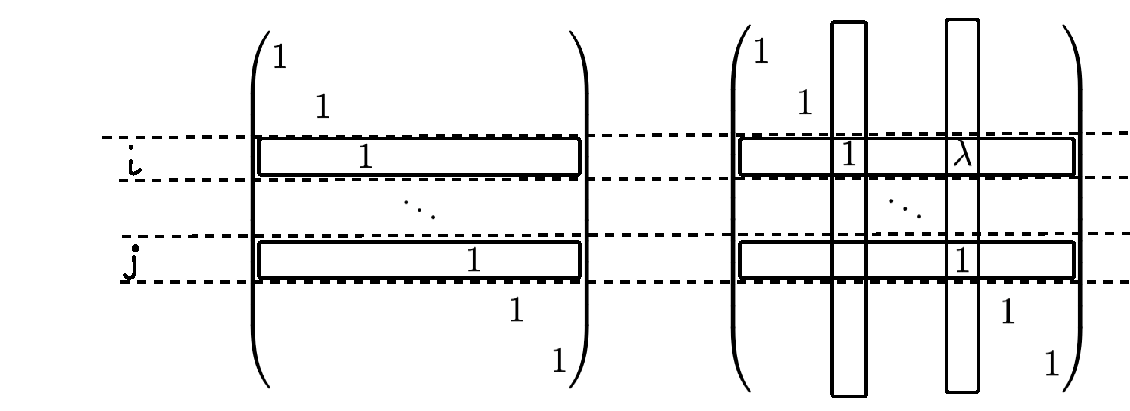
\includegraphics[width=12cm]{image/image8.2.1.pdf}$$
    ЭП2: $\overline{a_i} \leftrightarrow  \overline{a_j}, \ \ i \not = j$ \tab[2.5cm] ЭП3: $\overline{a_i} \leftrightarrow \mu \overline{a_i}, \ \ \mu \not = 0$ \\
    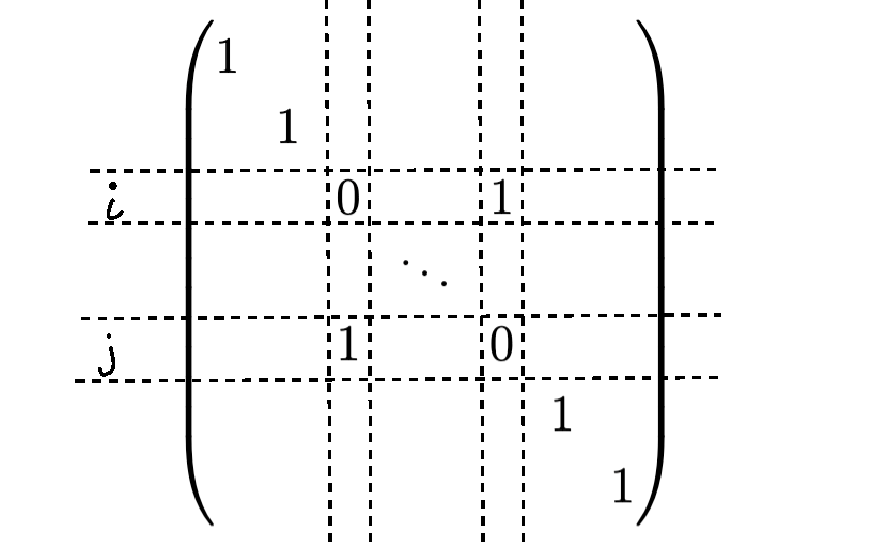
\includegraphics[width=7cm]{image/image8.2.2.pdf}
    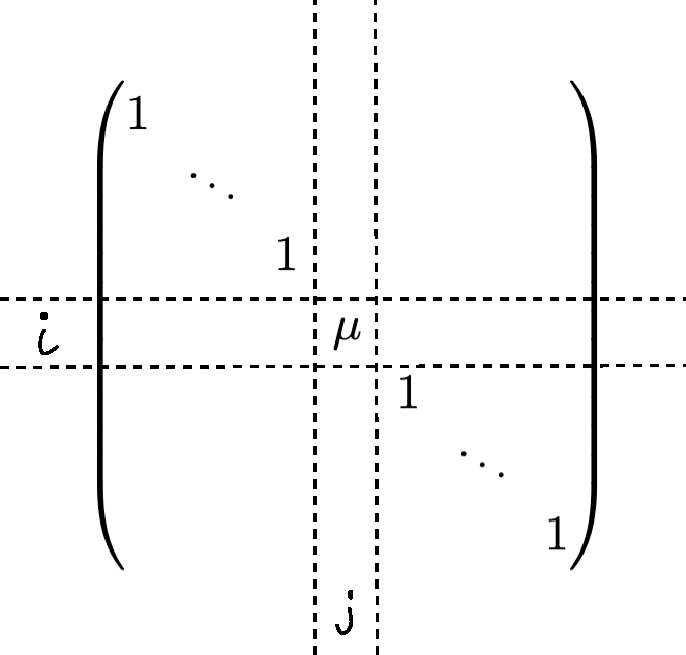
\includegraphics[width=5.6cm]{image/image8.2.3.pdf}
  \end{definition} 
  \setcounter{lemcount}{0}
  \begin{lemmanum} \label{lem8.1}\tab 
    \begin{itemize}
      \item[\textbf{1.1}] Любые ЭП над строками матрицы $A$ равносильно умножению матрицы $A$ слева на элементарную матрицу, т.е. \\
      $A \leadsto  \widetilde{A} \Longleftrightarrow \widetilde{A} = T \cdot A$ где $T$ - элементарная матрица, такая что $E \leadsto  T$
      \item[\textbf{1.2}] Любые ЭП над столбцами матрицы $A$ равносильно умножению матрицы $A$ справа на элементарную матрицу.
    \end{itemize}
  \end{lemmanum} 
  \begin{proof}
    Непосредственная проверка
  \end{proof}
  \begin{lemmanum} \label{lem8.2}
    Пусть $A$ - квадратная матрица порядка $n$, тогда:
    \begin{enumerate}
      \item Если $detA \not = 0$, то с помощью ЭП над строками, $A$ привести к $E$. 
      \item Если $detA = 0$, то с помощью ЭП над строками, в $A$ можно получить нулевую строку
    \end{enumerate}
  \end{lemmanum} 
  \begin{proof}
    Методом Гаусса любую матрицу можно привести к ступенчатому виду. Ступенчатый вид для квадратной матрицы является верхнетреугольной, т.е.:
    $$A \leadsto \widetilde{A} = \begin{pmatrix}
      \widetilde{a_{11}} & \null & * \\
      \null & \ddots & \null \\
      0 & \null & \widetilde{a_{nn}}
    \end{pmatrix}$$  
    $\Longrightarrow detA = \xi \cdot det \widetilde{A}$, где $\xi \not = 0$, \ $det \widetilde{A} = \widetilde{a_{11}} \cdot ... \cdot \widetilde{a_{nn}}$\\
    Итак, 
    $$detA =0 \Longleftrightarrow  det \widetilde{A} = 0 \Longleftrightarrow \widetilde{a_{11}} \cdot ... \cdot \widetilde{a_{nn}} =0$$ 
    \begin{enumerate}
      \item Если $detA \not = 0$, то $a_{11} \not = 0,...,a_{nn} \not = 0$ - лидеры матрицы $A$ \\ $\Longrightarrow \widetilde{A}$  приводится к улучшенному ступенчатому виду обратными ходом Гаусса и этот улучшенный ступенчатый вид совпадает с $E$
      \item Если $detA = 0$, то $a_{11} \cdot...\cdot a_{nn} = 0$ $\Longrightarrow  \exists k: a_{kk} = 0$. По определению ступенчатого вида $\forall i > k: \widetilde{a_{ii}} = 0 \Longrightarrow \widetilde{a_{nn}} = 0 \Longrightarrow$ последня строка в $\widetilde{A}$ нулевая.  
    \end{enumerate}
  \end{proof} 
  \begin{theoremnum}
    Пусть $A, B$ - квадратные матрицы порядка $n$, тогда: $$detAB = detA \cdot detB$$ 
  \end{theoremnum} 
  \begin{proof}
    Из ассоциативности умножения $T(AB) = (TA)B$, где $T$ элементарная матрица, получаем, что элементраное преобразование над строками матрицы $A$ соответствует элементарному преобразованию строк матрицы $AB$.  
    \begin{itemize}
      \item[1 случай.] $detA = 0$ (по лемме\eqref{lem8.1}, пункт 2)$\Longrightarrow A\leadsto \widetilde{A}$( с нулевой строкой) \\
      $\Longrightarrow \widetilde{A} = \cdot(T_1 \cdot ... \cdot T_k)\cdot A, \ $ где $T_i$ - матрицы элементарных преобразований. \\
      $\Longrightarrow (T_1 \cdot ... \cdot T_k)(AB) = ((T_1 \cdot ... \cdot T_k)A)B = \widetilde{A}B$ $\Longrightarrow det AB =0$, т.к. $AB \leadsto \widetilde{A}B$ 
      \item[2 случай.] $detA \not =$ 0 (по лемме\eqref{lem8.1}, пункт 1) $\Longrightarrow A\leadsto E \Longrightarrow E=(T_1 \cdot ... \cdot T_k)A$, \ где $T_i$ - матрицы элементарных преобразований. \\
      $(T_1 \cdot ... \cdot T_k)(AB) = ((T_1 \cdot ... \cdot T_k)A)B = EB = B$ \\
      $\Longrightarrow detAB = c \cdot det((T_1 \cdot ... \cdot T_k)AB) = c \cdot detB$  \\
      Рассмотрим отношение: $$\frac{detAB}{detA} = (*) $$ 
      $\\$ Произведем над матрицей $A$ ЭП, которые приведут матрицу $A \leadsto E$, одновременно производим такие же ЭП над $AB$. 
       $$ (*) = \frac{detEB}{detE} = detB$$ 
    \end{itemize}
  \end{proof} 
  \begin{theoremnum}
    (Об определителе с углом нулей) \\ Пусть $A$ - квадратная матрица порядка $k$ \\
    \tab[1.45cm]$B$ - квадратная матрица порядка $m$ \\
    \tab[1.45cm]$C$ - матрица размера $k \times m$. \\
    Тогда:
    $$det \begin{pmatrix}
      A & \vline & C \\
      \hline
      0 & \vline & B
    \end{pmatrix}(*) = detA \cdot detB$$ 
  \end{theoremnum} 

  \begin{proof} \tab
    \begin{itemize}
      \item[1 случай.] $detB = 0$ \\
      (По лемме \eqref{lem8.2}, пункт 2) $B\leadsto \widetilde{B}$ 
      Производя точно такие же ЭП над последними $m$ строками матрицы $(*)$ , получаем нулевую строку $$\Longrightarrow det \begin{pmatrix}
        A & \vline & C \\
        \hline
        0 & \vline & B
      \end{pmatrix} = detA \cdot detB = 0$$  
      \item[2 случай.] $detA = 0$ Аналогично как в 1 случае, только ЭП над столбцами. 
      \item[3 случай.] $detA \not = 0, detB \not = 0$ \\
      Рассмотрим отношение:
      $$\frac{det \begin{pmatrix}
        A & \vline & C \\
        \hline
        0 & \vline & B
      \end{pmatrix} = detA \cdot detB}{detA \cdot detB}$$\\ (По лемме \eqref{lem8.2}, пункт 1) $A\leadsto E$, $B\leadsto E$ \\
      Преобразуем матрицу $A$ с помощью ЭП над стролбцами, которые приводят $A \leadsto E$, преобразуем $B$ с помощью ЭП над строками, которые приводят $B \leadsto E$. Одновременно преобразуем матрицу $(*)$ с помощью таких же ЭП над строками и столбцами, отношение при этом не изменится. \\
      Тогда: 
      $$\frac{det \begin{pmatrix}
        A & \vline & C \\
        \hline
        0 & \vline & B
      \end{pmatrix}}{detA \cdot detB} =
      \frac{det \begin{pmatrix}
        E & \vline & C \\
        \hline
        0 & \vline & E
      \end{pmatrix}}{detE \cdot detE} = 1$$    
    \end{itemize}
  \end{proof} 

  \subsection{Разложение определителя по строке}

  $A$ - матрица размера $m \times n$. \\ 
  $i_1,...,i_k$ - номера некоторого разложения строк в $A$. \\ $j_1,...,j_t$ - номера некоторого разложения столбцов в $A$.
  \begin{definition}
    Матрица, состоящая из элементов матрицы $A$, стоящих на пересечении строк с номерами $i_1,...,i_k$ и столбцов с номерами $j_1,...,j_t$, называется подматрицей матрицы $A$\\
    Обозначение: 
    $A \begin{matrix}
      i_1 & \cdots & i_s \\
      \vdots & \null & \vdots \\
      j_1 & \cdots & j_t
    \end{matrix}$ 
  \end{definition}  
  \begin{definition}
    Минорами $k-$ого порядка матрицы $A$ называется определитель квадратной подматрицы порядка $k$. 
  \end{definition} 
  
  \begin{example1}
    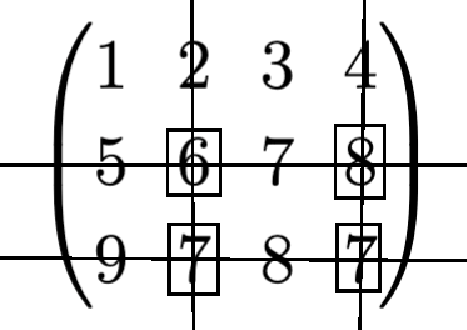
\includegraphics[width=3cm]{image/image8.3.1.pdf} $\Longrightarrow \text{Минор}= \begin{vmatrix}
      6 & 8 \\ 7 & 7
    \end{vmatrix}$ 
  \end{example1}
  Пусть $A$ квадратная матрица порядка $n$ 
  \begin{definition}
    Минор порядка $(n-1)$ квадратной матрицы $A$, полученный вычеркиванием $i-$ой строки и $j-$ого столбца, называется дополнительным минором к элементу $a_{ij}$.  \\
    Обозначается: $M_{ij}$ 
  \end{definition}
  \begin{example1}
    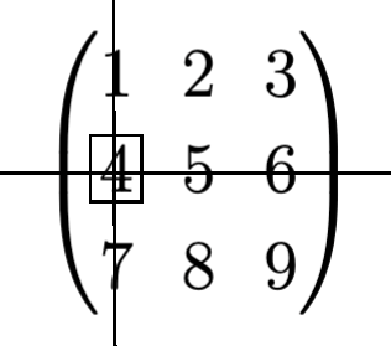
\includegraphics[width=3cm]{image/image8.3.2.pdf}$\Longrightarrow M_{12}= \begin{vmatrix}
      2 && 3 \\ 8 && 9
    \end{vmatrix} = -6$ 
  \end{example1}
  
  \begin{definition}
    Алгебраческое дополнение к элементу $a_{ij}$ - это число: $$A_{ij} = (-1)^{i+j} \cdot M_{ij}$$ 
  \end{definition} 
  \begin{example1}
    (к прошлому примеру) $A_{21} = (-1)^{2+1}(-6) = 6$  
  \end{example1}

  % \textbf{Мораль в том, что я не успел....}
   
\end{document}


